\documentclass[12pt,letterpaper]{report}

\marginparsep 0pt
\textwidth 6in
\topmargin 0pt
\headsep .5in
\textheight 9.2in
\voffset = 0pt
\hoffset = 0pt
\marginparwidth = 0pt \oddsidemargin = 0pt \sloppy

%Dimensiones de la página
\usepackage[left=2.5cm,top=3cm,right=2.5cm,bottom=2.5cm]{geometry}
%Sangría
\setlength{\parindent}{1cm}

%Numeracion
\pagenumbering{arabic}
\usepackage{graphicx}    % ya lo tendrás cargado
\usepackage{adjustbox}   % añade \adjustbox{}
\usepackage{tikz}
\usepackage{template}
\usepackage{amsmath,amsfonts}
\usepackage{graphicx}
\usepackage{graphics}
\usepackage[dvips]{epsfig}
\usepackage{times}
\usepackage[utf8]{inputenc}
\usepackage[dvips]{graphicx}
\usepackage[dvipsnames]{xcolor}
\usepackage[spanish]{babel}
\newcommand{\ie}{i.e.}
\newcommand {\out}[1]{}
\newtheorem{definicion}{Definicion}
\usepackage[dvips]{epsfig}
\usepackage{rotating}
\usepackage{multirow}
\usepackage{array}
\usepackage{longtable}
\usepackage[]{fontenc}
\usepackage{hyperref}
\usepackage{float}
\usepackage{tabularx}
\usepackage{booktabs}
\renewcommand{\shorthandsspanish}{}

\addto\captionsspanish{
\def\listtablename{Índice de tablas}
\def\tablename{Tabla}}

\sloppy

\begin{document}
\title{\textbf{Herramienta de apoyo automática en la estimación del estadio de heridas ulcerosas en pacientes con pie diabético}}
\author{\textbf{Benjamin Alejandro Morales Carvajal}}
\principaladviser{Ana Aguilera Faraco}
\coprincipaladviser{Julio Sotelo Parraguez, Marcelo Marquez}


\beforepreface
\prefacesection{Resumen}

Las heridas ulcerosas en pacientes con pie diabético representan una complicación clínica de alta prevalencia y riesgo, que afecta la calidad de vida de los pacientes y genera elevados costos sanitarios. Tradicionalmente, su evaluación depende de criterios visuales subjetivos, lo que provoca variabilidad diagnóstica y retrasos en las decisiones terapéuticas; aunque se utiliza la escala PWAT (Photographic Wound Assessment Tool), esta aún presenta limitaciones en objetividad y automatización.

Para abordar esta problemática, se desarrolla una herramienta automatizada que integra un modelo avanzado de segmentación de imágenes\,\footnote{También denominada \emph{segmentación semántica}, consiste en clasificar cada píxel según la región que representa.}, extracción de características radiómicas mediante pyradiomics y algoritmos de \textit{machine learning}, complementados con información clínica adicional para estimar objetivamente el puntaje PWAT.

Los resultados demuestran una mejora significativa en precisión y reproducibilidad frente a métodos manuales, posibilitando una evaluación integral del paciente y promoviendo intervenciones clínicas más oportunas y eficientes. De este modo, la metodología aporta robustez y escalabilidad al estado del arte en la valoración de heridas ulcerosas.

En un contexto más amplio, la herramienta contribuye a reducir complicaciones graves, optimizar la asignación de recursos sanitarios y mejorar la atención sanitaria general; a futuro, su implementación en aplicaciones móviles podría ampliar el acceso a evaluaciones remotas y generar alertas tempranas de deterioro.
%A continuación aspectos que debe considera para escribir un resumen comprensible y que cumpla su %propósito.
%
%\begin{itemize}
%    \item Una o dos oraciones que provean una introducción básica al área de trabajo, comprensibles %para un interesado de cualquier disciplina.
%    \item Dos o tres oraciones de antecedentes más detallados, comprensibles para personas de %disciplinas relacionadas.
%    \item Una oración que aclara el problema general que trata en este trabajo de título.
%    \item Una oración que resume el resultado principal.
%    \item Dos o tres oraciones que expliquen el aporte de sus resultados al estado del arte.
%    \item Una o dos oraciones para situar los resultados en un contexto más general.
%    \item (opcional) Dos o tres oraciones para proporcionar una perspectiva más amplia, fácilmente %comprensible para una persona de cualquier disciplina.
%
%\end{itemize}
%Recuerde 
%\begin{itemize}
%    \item El resumen es una consolidación de su trabajo.
%    \item Debe ser conciso y describir el alcance de su trabajo, resumir sus resultados y presentar %las principales conclusiones. 
%    \item Debe tener máximo 250 palabras. 
%    \item Debe ser escrito en pasado. 
%    
%\end{itemize}
%
%\textit{Importante: Tome los elementos que sean pertinentes a la etapa en que está de su trabajo de título. Estos aspectos están pensados para su documento final.}
%\newpage
%\prefacesection{Agradecimientos}
%Aqui pueden colocar sus agradecimientos.
%Si han estudiado con becas es recomendable colocar los agradecimientos a las instituciones que les otorgaron las becas.

%\afterpreface

\tableofcontents
\newpage

%%=============================================================================
%% List of Figures

%\renewcommand{\listfigurename}{List of Figures}
\listoffigures
\newpage

%%=============================================================================
%% List of Tables
\renewcommand{\listtablename}{Índice de tablas} 
\renewcommand{\tablename}{Tabla} 

\listoftables
\newpage

\pagenumbering{arabic}

%Aquí deben incluir el fuente de cada capítulo, sin su encabezado:

\chapter{Introducci\'on}
\label{ch:Intro}

\section{Introducción}
\label{sec:Intr}

La diabetes mellitus es reconocida mundialmente como uno de los principales desafíos sanitarios del siglo XXI, debido a su elevada prevalencia -- que se a duplicado entre 2003 y 2016-2017, pasando de un 6,4\% a un 12,3\%  de la poblacion en la Encuesta Nacional de Salud (ENS) \cite{troncoso2020estilos} -- y a las múltiples complicaciones asociadas que afectan significativamente la calidad de vida de los pacientes, así como los costos para los sistemas de salud \cite{ministerio2022estrategia}. Esta enfermedad crónica no solo genera un impacto directo sobre quienes la padecen, sino también sobre sus familias y comunidades, debido al manejo continuo y a largo plazo que exige. Entre dichas complicaciones, las ulceras en pacientes con pie diabetico destacan por su alta incidencia, gravedad clinica y complejidad terapeutica. Estas lesiones suponene una carga considerable para los sistemas de salud, dada su tendencia a la cronicidadm las frecuentes recaidas y el riesgo elevado de infecciones graves que, en muchos casos, culminan en amputaciones subsecuentes. De hecho, las heridas en pie diabetico son una de las principales causas de hospitalización prolongada y discapacidad permanente en estos pacientes \cite{mishra2017diabetic,bandyk2018diabetic}.

La evolucion clinica de las heridas ulcerosas en pie diabetico depende en gran medida de criterios visuales subjetivos, lo que genera inconsistencias diagnosticas y retrasos en  la toma de decisiones terapeuticas oportunas. La falta de criterios cuantitativos y estandarizados dificulta la comparacion entre distintos profesionales y centros, y retrasa la optimizacion temprana de los tratamientos. Este retraso agrava el pronostico y eleva el coste asistencial, pues las ulceras que no cicatrizan en las primeras cuatro semanas se cronifican con mas facilidad y requieren intervenciones mas invasivas y costosas \cite{mishra2017diabetic,bandyk2018diabetic}. Por ello, resulta imprescindible avanzar hacia metodos de evaluacion que integren herramientas objetivas -- capaces de monitorizar el tamaño, la profundidad y la composicion tisular de la lesion -- y que ofrezcan un apoyo real a la decision clinica. En este contexto, la inteligencia artificial aplicada al analisis de imagenes y la automatizacion de escalas de valorizacion como Photographic Wound Assessment Tool (PWAT) \cite{thompson2013reliability} representan una via prometedora para mejorar la precision, la reproducibilidad y la rapidez en el seguimiento de la cicatrizacion.

Paralelamente, esta problemática se encuentra agravada por el fenómeno de la multimorbilidad, definida como la coexistencia de dos o más condiciones crónicas en un mismo individuo, lo cual implica un incremento sustancial en la complejidad clínica y la carga asistencial, demandando enfoques integrales y basados en evidencia que optimicen los resultados en salud \cite{sarmiento2022patrones}.

En respuesta a este contexto, surge la necesidad de desarrollar herramientas objetivas y cuantitativas para mejorar el seguimiento y la evaluación del proceso de cicatrización en heridas ulcerosas del pie diabético. Esta investigación y desarrollo propone enfrentar dicha necesidad mediante el desarrollo de una herramienta automatizada que estime objetivamente el estadio de estas heridas a partir de técnicas avanzadas de procesamiento de imágenes y aprendizaje automático. La herramienta propuesta integrará métodos de segmentación automática de heridas utilizando imágenes capturadas mediante dispositivos móviles, la extracción y análisis de características radiómicas empleando técnicas especializadas como pyradiomics \cite{van2017computational}, y algoritmos avanzados de machine learning para una estimación precisa del estadio clínico según la escala PWAT (Photographic Wound Assessment Tool) \cite{thompson2013reliability}. Además, se contemplará la incorporación de información clínica relevante del paciente mediante registros digitales, buscando así una evaluación integral que permita una gestión clínica más eficiente.

De esta manera, la implementación de esta herramienta busca mejorar significativamente la precisión diagnóstica, reducir complicaciones mayores, favorecer intervenciones oportunas y eficientes, y optimizar el uso de recursos sanitarios disponibles, respondiendo así efectivamente a un desafío sanitario de creciente relevancia global \cite{organizacion2016informe}.

\chapter{Marco Conceptual y Estado del Arte}
\label{ch:MC}
                

\section{Marco Conceptual}
\label{sc:MC}


Las heridas cr'onicas del pie diab'etico presentan cicatrizaci'on prolongada y alto riesgo de complicaciones. Se clasifican por gravedad mediante escalas como Wagner o PWAT y evolucionan a trav'es de fases inflamatoria, proliferativa y de remodelaci'on, afectadas por la multimorbilidad propia de estos pacientes. Pese a estos sistemas, la evaluaci'on sigue siendo manual y dependiente del especialista, lo que motiva aplicar visi'on por computador y aprendizaje autom'atico para cuantificar la lesi'on de forma objetiva.



\section{Estado del Arte}
\label{sc:EA}


Las heridas crónicas, como las úlceras diabéticas del pie , representan un serio problema de salud mundial por su alta prevalencia y complicaciones. Se estima que entre un 19\% y 34\% de los pacientes diabéticos desarrollarán una úlcera de pie en su vida, con elevado riesgo de mala cicatrización, amputación de miembros inferiores e incluso reducción de la supervivencia \cite{Zhang2022}. Las úlceras por presión (escaras) y las úlceras venosas son otros tipos comunes de heridas crónicas, todas contribuyendo a costos sanitarios multimillonarios \cite{Wang2020,Sendilraj2024}. La evaluación clínica de estas lesiones suele basarse en la inspección visual y mediciones manuales, procesos sujetos a la experiencia del profesional y, por tanto, con variabilidad interobservador \cite{Curti2024}. Para estandarizar la valoración, se han propuesto escalas clínicas como \textbf{BWAT}, \textbf{PUSH} o la clasificación de \textbf{Wagner}, entre otras. Sin embargo, aplicarlas requiere tiempo y puede ser subjetivo. En la última década, la \textbf{inteligencia artificial} (IA) – especialmente técnicas de \textbf{machine learning} (ML) y \textbf{deep learning} (DL) – ha emergido como herramienta prometedora para automatizar la evaluación de heridas ulcerosas, buscando mayor objetividad, eficiencia y seguimiento continuo \cite{Sendilraj2024,Curti2024}.

A continuación, se presenta una revisión crítica de trabajos relevantes (2015–2025) sobre el uso de IA en la evaluación automática de heridas ulcerosas, con énfasis en pie diabético pero sin limitarse a este. Se abordan desarrollos en segmentación de imágenes (delimitación de la herida y análisis de tamaño), clasificación y gradación de severidad, análisis de tejidos en la herida, predicción de evolución de la cicatrización, así como enfoques multimodales. Se comparan metodologías, resultados, conjuntos de datos empleados, fortalezas, debilidades y posibles mejoras, organizando la información en secciones temáticas para facilitar su lectura.

\subsection{Escalas clínicas de evaluación de heridas}

En la práctica clínica, existen escalas estandarizadas para evaluar el estado y la evolución de heridas. Por ejemplo, \textbf{BWAT (Bates-Jensen Wound Assessment Tool)} consta de 13 ítems que evalúan características como:
\begin{enumerate}
    \item tamaño
    \item profundidad de la herida
    \item bordes
    \item presencia de socavamiento
    \item tipo de tejido necrotico
    \item cantidad de tejido necrotico
    \item cantidad de tejido de ganulacion
    \item cantidad de tejido de epilizacion
    \item tipo de exudado
    \item cantidad de exudad
    \item condicion de la piel peilesional - color
    \item condicion de la piel peilesional - edema
    \item condicion de la piel peilesional - induracion
    
\end{enumerate}
Cada ítem se puntúa de 1 (mejor situación) a 5 (peor), ofreciendo un puntaje total que cuantifica la gravedad de la herida. Debido a que varios ítems requieren examen directo (ej., medir profundidad o socavamientos manualmente), el \textbf{BWAT} tradicionalmente se aplica \textbf{en persona} durante la visita clínica . Esto dificulta su automatización posterior a partir de fotografías, pues algunas características no son discernibles solo con imágenes. Para solventar esa limitación, se introdujo la escala \textbf{PWAT} \cite{Curti2024}. 

El PWAT es una adaptación del BWAT que incluye solo un subconjunto de los ítems –aquellos inferibles directamente de una fotografía–, excluyendo por ejemplo la profundidad o socavamientos. Pese a ser más limitado, el PWAT ha demostrado \textbf{validez y robustez} en aplicaciones clínicas para seguimiento mediante imágenes . Otra escala común es la \textbf{PUSH (Pressure Ulcer Scale for Healing)}, diseñada por NPIAP para monitorizar la cicatrización de úlceras por presión, combinando medidas de área superficial de la herida, cantidad de exudado y tipo de tejido dominante en el lecho ulceroso (granulación, esfacelo/fibrina o epitelial). La PUSH genera un puntaje total que disminuye a medida que la herida cura, facilitando evaluar si una úlcera por presión está mejorando o no

En cuanto a clasificación de severidad, para las úlceras de pie diabético se emplea la \textbf{clasificación de Wagner}, de 6 niveles (0 a 5) que describen la profundidad y complicaciones de la lesión . Un Wagner 0 indica pie de riesgo sin ulceración; Wagner 1 es una úlcera superficial; Wagner 2 implica extensión a tendón, hueso o cápsula articular; Wagner 3 añade infección grave (ej. osteomielitis o absceso); Wagner 4 denota gangrena localizada (por isquemia/infección) en antepié o talón; y Wagner 5 es gangrena extensa de todo el pie, generalmente requiriendo amputación \cite{Girmaw2025}. Esta clasificación guía el manejo clínico del pie diabético y pronostica la necesidad de intervenciones mayores.

Aunque las escalas estandarizadas han reducido parcialmente la subjetividad, sigue habiendo variabilidad entre observadores al aplicarlas. Por ejemplo, dos médicos podrían discrepar en la estimación del porcentaje de tejido de granulación vs. esfacelo en un lecho ulceroso, afectando la puntuación BWAT. En efecto, la evaluación en forma de escalas Likert impone categorías que \textbf{fuerzan la cuantificación} de rasgos de la herida, pero la interpretación visual sigue siendo del clínico . Estudios reportan que persiste una variabilidad inter e intraobservador no desdeñable incluso utilizando herramientas estandarizadas . Esto ha motivado la investigación en sistemas automatizados que extraigan de imágenes métricas objetivas de la herida (dimensiones, tipos de tejido, etc.) para calcular o apoyar estas escalas. A continuación se revisan los avances en dichos sistemas basados en IA.

Segmentar una herida en una imagen consiste en delinear automáticamente el contorno de la lesión y separarla de la piel sana circundante. Es un paso fundamental, pues permite calcular la superficie de la úlcera, un parámetro clave para monitorear la cicatrización (una reducción del área a lo largo del tiempo suele indicar progreso) \cite{Wang2020}. La medición manual del área (ej., con reglas o calcos sobre la herida) es engorrosa, imprecisa y consume tiempo \cite{Filko2023}. Automatizar la segmentación permite obtener \textbf{medidas objetivas de forma rápida}, facilitando la documentación y seguimiento en historias clínicas electrónicas . 

\begin{itemize}
    \item \textbf{Enfoques tradicionales}
    \begin{itemize}
        \item Antes del auge del deep learning, se exploraron métodos de visión por computador clásica para segmentar heridas crónicas. Estos incluían técnicas como umbralización de color, detección de bordes, crecimiento de regiones y uso de clasificadores basados en características diseñadas manualmente. Por ejemplo, Wang \cite{Chemello2022} propusieron un método de dos etapas: primero se sobresegmenta la imagen en superpixels y se extraen múltiples descriptores de color y textura; luego, un conjunto de clasificadores SVM distingue superpixels de herida vs. piel . Este clasificador en cascada logró sensibilidad $\sim73.3\%$ y especificidad $\sim94.6\%$ en segmentar úlceras diabéticas (100 imágenes de 15 pacientes) , superando a enfoques de una sola etapa o redes neuronales poco profundas probadas en esa cohorte. Posteriormente, Wang \cite{Chemello2022}  abordaron el reto de la variabilidad en condiciones de captura (iluminación, ángulo, fondo) entrenando un modelo de Random Field jerárquico (AHRF) que extendía los Conditional Random Fields. Probado en un conjunto pequeño de imágenes sintéticas y reales, este modelo logró especificidad >95\% y sensibilidad >77\% , mostrando mejor desempeño que CRFs tradicionales. Los autores sugirieron que en escenarios con muy pocos datos, modelos probabilísticos como AHRF podrían superar a CNNs profundas, aunque anticiparon que con más datos las redes neuronales lograrían resultados superiores .
    \end{itemize}
    \item \textbf{Deep learning en segmentación}
    \begin{itemize}
        \item A medida que aumentaron los conjuntos de datos de heridas, los métodos de deep learning demostraron ventajas claras en segmentación. Diversos arquitecturas de segmentación semántica han sido aplicadas: Fully Convolutional Networks, U-Net, SegNet, etc. Ohura evaluaron redes para segmentar úlceras combinando datos de distintos tipos de heridas: entrenaron CNNs (SegNet, LinkNet, U-Net) principalmente con 400 imágenes de úlceras por presión y apenas 20 imágenes de UPD \cite{Chemello2022}. Sorprendentemente, la U-Net logró altísima precisión al segmentar incluso las úlceras diabéticas (especificidad 0.943 y sensibilidad 0.993 en promedio) , evidenciando que patrones aprendidos en úlceras por presión podían transferirse a otras etiologías crónicas con morfologías parecidas. Este resultado sugirió que, dadas suficientes imágenes de entrenamiento, las redes profundas segmentan heridas con fiabilidad casi humana
        
        \item Varios grupos han construido sus propios datasets para entrenar modelos. Wang \cite{Wang2020} compilaron 1109 imágenes de úlceras de pie diabético de 889 pacientes y entrenaron un modelo basado en MobileNetV2 para segmentación automática . Eligiendo MobileNetV2 por su ligereza, demostraron que un modelo de baja complejidad podía lograr un rendimiento equiparable a redes más profundas en esa tarea . La arquitectura propuesta combinaba la segmentación por CNN con un post-procesamiento de componentes conexos para afinar la máscara final . Gracias a su menor costo computacional, este enfoque apuntaba a implementaciones en dispositivos móviles sin sacrificar precisión. De hecho, otras investigaciones también resaltan la factibilidad de ejecutar modelos de segmentación en smartphones: Ramachandram \cite{Ramachandram2022} entrenaron modelos U-Net con el mayor conjunto publicado hasta la fecha ($\approx465$ mil pares de imagen-máscara para segmentar heridas, más 17 mil para segmentar tejidos dentro de la herida) obtenidos de la base de datos de la compañía Swift Medical . El modelo resultante segmenta en tiempo casi real en un teléfono, dada la optimización lograda con ese enorme dataset . En pruebas, su red alcanzó un IoU promedio de 0,8644 delimitando el área de la herida (muy alto acuerdo con el contorno verdadero). Incluso en condiciones de iluminación y piel variadas, la segmentación automática mostró ser robusta y sin sesgos por tono de piel – un aspecto importante para equidad clínica

        \item La precisión de la segmentación profunda se refleja también en desafíos internacionales. En la competencia Diabetic Foot Ulcer Challenge (DFUC2020), múltiples equipos aplicaron detectores y segmentadores basados en YOLO, Faster R-CNN y U-Net. Un resumen de Yap et al. reportó que las mejores refinaciones de YOLOv3 lograron $\sim 91.95\%$ de exactitud en detección de úlcera en imagen completa, y variantes de Faster R-CNN alcanzaron hasta 91.4\% mAP . Para segmentación semántica, arquitecturas tipo U-Net destacaron; en un estudio se informa que un modelo U-Net superó a otras arquitecturas con 94.96\% de precisión en segmentación de la herida . Asimismo, aplicando Mask RCNN (que combina detección y segmentación a nivel de instancia) se han logrado valores de precision $\sim 0.86$ y mAP $\sim 0.51$ segmentando úlceras . En suma, la comunidad ha validado que las CNN bien entrenadas pueden delimitar las heridas con alta fiabilidad, permitiendo calcular el área de forma automática y consistente
    \end{itemize}
    \item \textbf{Comparativa de enfoques de segmentación}
    \begin{itemize}
        \item Los métodos basados en DL superan a los clásicos en exactitud, especialmente cuando hay suficiente volumen de datos para entrenar. Los enfoques tradicionales (p. ej. SVM con atributos diseñados) alcanzaron especificidades altas en conjuntos pequeños , pero su sensibilidad quedaba limitada posiblemente por la variabilidad visual que no capturaban totalmente. Las CNN, al aprender características de bajo a alto nivel directamente de los píxeles, manejan mejor dicha variabilidad, logrando sensibilidades y especificidades cercanas al 90–99\% \cite{Chemello2022}. No obstante, un desafío común es la \textbf{generalización}: muchos estudios emplearon datos de un único centro o condiciones controladas, y un modelo puede perder precisión si se aplica a imágenes con distinta iluminación, dispositivos o poblaciones. Para mitigar esto, algunos autores integran pasos de pre-procesamiento de color (ej. conversión a espacios de color uniformes Lab, YCbCr) antes de la segmentación, como en la plataforma DFUCare \cite{Sendilraj2024}, o aplican extensas técnicas de \textit{data augmentation } \cite{Aldughayfiq2023} para expandir la diversidad de ejemplos de entrenamiento. Otra tendencia es combinar modalidades: Filko \cite{Filko2023} desarrollaron un sistema robótico que captura simultáneamente la herida en 2D (fotografía RGB) y en 3D mediante escaneo láser, usando una CNN 2D para segmentar inicialmente la herida en la imagen y luego refinando el contorno sobre la malla 3D con un modelo activo de contornos \cite{Filko2023}. Este enfoque híbrido produce un modelo 3D de la superficie herida, permitiendo medir \textbf{perímetro, área y volumen} de la úlcera de forma totalmente automática . La incorporación de volumen es valiosa, ya que una reducción volumétrica puede indicar curación antes que la reducción de área en ciertas lesiones profundas.
    \end{itemize}
\end{itemize}

\subsection{Clasificación de heridas: detección, severidad e infección}

Otra línea de aplicación de la IA en heridas es la clasificación automática, que puede tomar varias formas según el objetivo clínico:
\begin{itemize}
    \item \textbf{Detección vs. piel sana}
    \begin{itemize}
        \item Identificar si en una foto de un pie o de la piel hay una úlcera presente (clasificación binaria herida/no herida)
    \end{itemize}
    \item \textbf{Clasificación del tipo de herida}
    \begin{itemize}
        \item  Por etiología (diabética, venosa, por presión, quirúrgica, etc.) o por estadio (p. ej. estadios I–IV de úlcera por presión, grados Wagner 0–5 en pie diabético).
    \end{itemize}
    \item \textbf{Detección de signos clínicos en la herida}
    \begin{itemize}
        \item clasificar si una úlcera de pie diabético muestra signos de infección, de isquemia, ambas o ninguna (clasificación multinomial)
    \end{itemize}
    \item \textbf{Gradación de severidad}
    \begin{itemize}
        \item Asociada a escalas como Wagner, Texas, NPUAP, etc., a partir de la imagen.
    \end{itemize}
\end{itemize}

Varios trabajos han explorado redes neuronales para estas tareas de clasificación a nivel de imagen o de herida. En general, las arquitecturas de deep learning utilizadas son CNNs de clasificación (VGG, ResNet, EfficientNet, MobileNet, etc.) o detectores de objetos cuando se necesita localizar la herida en la foto además de clasificarla

\begin{itemize}
    \item \textbf{Detección de úlceras (binario sí/no)}
    \begin{itemize}
        \item Goyal \cite{Goyal2020} desarrollaron \textbf{DFUNet}, una arquitectura de CNN especializada en identificar regiones con úlcera vs piel normal en el pie diabético . DFUNet combinaba convoluciones profundas con capas paralelas y de distinta profundidad para captar características a múltiples escalas, logrando mejorar la discriminación entre piel sana y lesionada . Este trabajo pionero ya demostraba la viabilidad de deep learning para detectar automáticamente una úlcera en imágenes donde pudiera haber artefactos o variabilidad en los pies de pacientes diabéticos. Estudios posteriores han reportado precisiones muy altas en esta tarea: Cassidy \cite{Cassidy2023} hicieron un \textbf{estudio clínico multicéntrico} con 203 fotografías de pies tomadas con un smartphone de bajo costo, pasando cada imagen por un sistema de IA para detectar úlceras y comparando con la evaluación de especialistas. El modelo alcanzó \textbf{91.6\% de sensibilidad y 92.4\% de especificidad} en la detección de úlceras , prácticamente equiparable a la precisión humana. Es notable que incluso con imágenes capturadas en entornos reales (no de estudio), la IA mantuvo alto desempeño, lo cual avala su potencial uso como herramienta de tamizaje remoto. Los clínicos participantes mostraron además alto acuerdo (Kappa >0.8) en que el sistema identifica correctamente las úlceras . Este es uno de los primeros ensayos que prueban un algoritmo de visión computacional en campo con pacientes, marcando un hito hacia la adopción como dispositivo médico

        \item En escenarios más controlados, se han conseguido incluso accuracies cercanas a la perfección en detección binaria, aunque en conjuntos de datos limitados. Por ejemplo, Girmaw y Taye \cite{Girmaw2025} entrenaron un modelo MobileNetV2 para detectar la presencia de UPD y reportan \textbf{100\% de exactitud} en sus pruebas . Si bien este resultado es llamativo, es probable que su dataset no haya sido muy amplio ni diverso, lo que podría indicar cierto \textit{overfitting}. Aun así, refleja la capacidad de las CNN modernas: un modelo ligero fue suficiente para separar completamente imágenes con vs sin úlcera en el conjunto evaluado . Los autores destacan la importancia de la cuidadosa preparación de datos (anotaciones, aumentos, etc.) y ajuste de hiperparámetros para lograr tal rendimiento , subrayando que la clave está tanto en la arquitectura como en el \textit{fine-tuning} adecuado.
    \end{itemize}
        
\end{itemize}



\chapter{Definición del Problema }
\label{ch:Problema}
\usetikzlibrary{arrows,positioning}
\section{Definición del Problema}
\subsection{Problema}
\label{ssec:P}

La evaluación clínica actual del pie diabético está predominantemente basada en criterios visuales subjetivos, lo que genera importantes inconsistencias diagnósticas y retrasa la implementación de intervenciones clínicas oportunas y efectivas. Diversas investigaciones han señalado que esta subjetividad genera una significativa variabilidad inter e intraoperador, afectando negativamente el pronóstico y evolución clínica de los pacientes \cite{mishra2017diabetic, bandyk2018diabetic, thompson2013reliability}. Aunque existen herramientas como el Photographic Wound Assessment Tool (PWAT), diseñadas para reducir dicha subjetividad y mejorar la precisión diagnóstica mediante la evaluación de imágenes, aún persisten limitaciones en términos de implementación práctica, objetividad plena y automatización del proceso \cite{thompson2013reliability, organizacion2016informe}.

Recientemente, se han desarrollado diversos enfoques automatizados basados en inteligencia artificial y técnicas avanzadas de procesamiento de imágenes para mejorar la precisión y objetividad de estas evaluaciones. Sin embargo, muchas de estas propuestas todavía enfrentan dificultades relacionadas con la estandarización del proceso, la integración efectiva de información clínica adicional y la necesidad de dispositivos específicos o condiciones altamente controladas para la captura de imágenes \cite{van2017computational}. Un ejemplo relevante es el trabajo reciente de Curti \cite{Curti2024}, quienes presentaron una propuesta automatizada para la predicción del puntaje PWAT utilizando imágenes capturadas con smartphones y técnicas avanzadas de análisis radiómico y aprendizaje automático, logrando una alta correlación con las evaluaciones clínicas manuales \cite{Curti2024}. A pesar de este avance, se evidencian limitaciones como la dependencia de un conjunto limitado y monocéntrico de imágenes, la ausencia de condiciones estandarizadas de captura y la dificultad para una integración clínica directa y sencilla.

\subsection{Solución Propuesta}
\label{ssec:SP}

Considerando los hallazgos de la literatura y las limitaciones existentes, la solución propuesta en este trabajo se enfoca en desarrollar una herramienta automatizada robusta que supere dichas restricciones. Para esto, se integrará un modelo avanzado de segmentación automática de heridas ya desarrollado, capaz de identificar y delimitar con precisión el área de las lesiones y las zonas circundantes (peri‑lesión). Estas segmentaciones serán la base para extraer características radiómicas altamente informativas mediante técnicas especializadas como pyradiomics. Dichas características incluyen parámetros relacionados con la textura, morfología, color y variabilidad de la herida, elementos que tradicionalmente los clínicos evalúan de forma visual y subjetiva.

Posteriormente, se aplicarán técnicas avanzadas de aprendizaje automático (machine learning), con el fin de obtener estimaciones precisas y objetivas del puntaje PWAT. Se contemplarán diferentes algoritmos predictivos, con el propósito de seleccionar la aproximación más efectiva. Además, se integrará información clínica relevante proveniente de registros digitales del paciente, tales como datos demográficos, historial clínico, parámetros de laboratorio y otras variables asociadas a la condición clínica del individuo. La integración de estos datos adicionales permitirá mejorar considerablemente la precisión diagnóstica y asegurar una evaluación integral del paciente, facilitando así la toma de decisiones clínicas oportunas y fundamentadas en evidencia.

Finalmente, esta herramienta se implementará en una interfaz de usuario amigable, diseñada para ser fácilmente adoptada en la práctica clínica cotidiana, minimizando las barreras tecnológicas y asegurando una aplicabilidad clínica directa y efectiva.

\subsection{Importancia del trabajo}
\label{ssec:IT}

Desde un punto de vista científico y social, el presente trabajo es altamente relevante. Científicamente, este proyecto ofrece una significativa contribución en la integración y aplicación práctica de métodos avanzados como machine learning, análisis radiómico y procesamiento automático de imágenes en el ámbito clínico, especialmente en el manejo de heridas crónicas asociadas a diabetes. La aplicación efectiva de estas técnicas permitirá establecer una metodología de evaluación de heridas mucho más precisa y reproducible, lo cual representa un avance significativo frente a las técnicas tradicionales.

Desde la perspectiva social, la importancia radica en su potencial para mejorar considerablemente la calidad de vida de los pacientes con pie diabético, reduciendo el riesgo de complicaciones graves como infecciones recurrentes y amputaciones, que impactan profundamente en la autonomía y bienestar de los afectados. Además, al optimizar la precisión diagnóstica y promover intervenciones clínicas oportunas, esta herramienta podría reducir los costos sanitarios derivados de tratamientos prolongados y hospitalizaciones recurrentes, facilitando una gestión más eficiente de los recursos del sistema de salud. En suma, el desarrollo e implementación de esta propuesta contribuirá significativamente a un manejo clínico más eficaz, centrado en el paciente y basado en evidencia científica robusta, con beneficios directos para individuos, comunidades y sistemas sanitarios en general.







\chapter{Objetivos}
\label{ch:OG}
\input{objetivos}

\chapter{Metodologia}
\label{ch:Met}
\input{metodologia}

\section{Planificación}
\label{ch:Plan}
\input{planificacion}

\chapter{Especificación de Requerimientos}
\label{ch:req}
\section{Especificación de Requerimientos}
\label{sc:ER}

Este sistema tiene como propósito apoyar al personal clínico en la estimación automática del estadio de heridas ulcerosas en pacientes con pie diabético, utilizando imágenes médicas procesadas mediante técnicas de segmentación, extracción de características radiómicas y modelos de predicción basados en aprendizaje automático.


\subsection{Requerimientos Funcionales}
\label{ssc:RF}

\begin{itemize}
    \item \textbf{RF1: Registro de usuario.} El sistema debe permitir registrar nuevos usuarios en la tabla \texttt{user}, incluyendo su RUT, nombre, correo, contraseña, rol y fecha de nacimiento.

    \item \textbf{RF2: Gestión de pacientes.} El sistema debe permitir al personal clínico registrar y actualizar información de pacientes en la tabla \texttt{paciente}, asociando cada paciente a un usuario y a un profesional responsable.

    \item \textbf{RF3: Registro de profesionales.} El sistema debe permitir registrar y administrar profesionales clínicos en la tabla \texttt{profesional}, vinculando cada uno a un usuario registrado.

    \item \textbf{RF4: Carga de imágenes clínicas.} El sistema debe permitir subir imágenes de heridas ulcerosas, guardando su nombre, fecha de captura, ruta de almacenamiento y asociación con el paciente correspondiente en la tabla \texttt{imagen}.

    \item \textbf{RF5: Segmentación de imágenes.} El sistema debe permitir registrar los resultados de segmentación de una imagen, especificando el método usado (manual o automática), la ruta de la máscara y la fecha de creación, en la tabla \texttt{segmentacion}.

    \item \textbf{RF6: Evaluación del estadio de la herida.} El sistema debe permitir registrar el puntaje PWAT calculado por modelo o experto humano en la tabla \texttt{pwatscore}, vinculando los resultados con una imagen y su segmentación correspondiente.

    \item \textbf{RF7: Visualización de evaluaciones.} El sistema debe permitir consultar el historial de evaluaciones PWAT asociadas a un paciente, visualizando fecha, evaluador, observaciones, imagen relacionada y resultados por categoría (JSON).

    \item \textbf{RF8: Validación cruzada de evaluaciones.} El sistema debe permitir comparar las evaluaciones realizadas por el modelo con aquellas realizadas por expertos clínicos sobre la misma imagen.

    \item \textbf{RF9: Gestión de acceso por rol.} El sistema debe restringir el acceso a funcionalidades según el campo \texttt{rol} de la tabla \texttt{user}, permitiendo, por ejemplo, que sólo usuarios con rol \texttt{doctor} o \texttt{enfermera} puedan ingresar evaluaciones clínicas.

\end{itemize}



\subsection{Requerimientos No Funcionales}
\label{ssc:RNF}

\begin{itemize}
    \item \textbf{RNF1:} El sistema debe procesar una imagen y mostrar el resultado en un tiempo máximo de 5 segundos.
    
    \item \textbf{RNF2:} El sistema debe ser portable y permitir escalabilidad horizontal mediante contenedores Docker, de forma que se puedan ejecutar multiples instancias concurrentes
    
    \item \textbf{RNF3:} El sistema debe tener una disponibilidad mínima del 99.5\% mensual.
    
    \item \textbf{RNF4:} El sistema debe utilizar cifrado TLS 1.2 o superior para la transmisión de imágenes y datos clínicos.
    
    \item \textbf{RNF5:} La interfaz de usuario debe ser intuitiva y responsiva, compatible con dispositivos móviles y navegadores modernos.
    
    \item \textbf{RNF6:} El código del sistema debe estar modularizado y documentado, facilitando su mantenimiento evolutivo y correctivo.
    
    \item \textbf{RNF7:} El sistema debe ser compatible con las tres últimas versiones de los navegadores Chrome, Firefox, Safari y Edge.
    
    \item \textbf{RNF8:} El backend debe permitir la interoperabilidad entre servicios desarrollados en Node.js y scripts Python, mediante APIs REST o invocaciones asincrónicas.
    
    \item \textbf{RNF9:} Cada predicción debe ser registrada con un identificador único y metadatos asociados (timestamp, parámetros utilizados, resultado) para permitir trazabilidad clínica y técnica.
\end{itemize}


\section{Funcionalidades del Sistema}
\label{sc:FS}


\subsection{Diagramas de Casos de Uso}
\label{ssc:DCU}

\begin{figure}[H] %si cambia la "H" por "t", se fuerza a que la figura quede arriba de la página
    \centering
    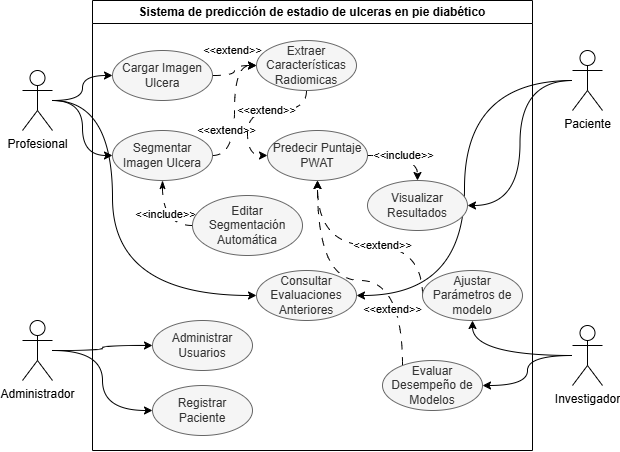
\includegraphics[width=1.1\textwidth]{imagenes/casosdeuso.drawio.png}
    \caption{Diagrama de casos de uso}
    \label{fig:scrum}
\end{figure}


\subsection{Casos de Uso (resumidos)}
\label{ssc:CUresumido}

\begin{table}[H]
  \small
  \centering
  \caption{Resumen condensado de Casos de Uso}
  \label{tab:cu_resumido}
  \begin{tabular}{p{1cm} p{6cm} p{2cm} p{4cm}}
    \toprule
    \textbf{ID} & \textbf{Descripción}                          & \textbf{Actor(es)}           & \textbf{Relación}           \\
    \midrule
    CU01        & Carga imagen de la úlcera                     & Profesional                  & Extiende CU02               \\
    CU02        & Extrae características radiomédicas           & Profesional                  & Depende de CU01             \\
    CU03        & Segmenta la imagen de la úlcera               & Profesional                  & Depende de CU01             \\
    CU04        & Edita segmentación automática                 & Profesional                  & Extiende CU03               \\
    CU05        & Visualiza resultados (PWAT)                   & Profesional, Paciente        & Incluye CU03, CU06          \\
    CU06        & Calcula y guarda puntaje PWAT                 & Profesional                  & Depende de CU03             \\
    CU07        & Consulta historial de evaluaciones            & Profesional, Paciente        & Depende de CU06             \\
    CU08        & Gestiona registro de paciente                 & Administrador                & –                           \\
    CU09        & Gestiona usuarios                             & Administrador                & –                           \\
    CU10        & Ajusta parámetros del modelo predictivo       & Investigador                 & Depende de CU06             \\
    CU11        & Evalúa desempeño del modelo                   & Investigador                 & Depende de CU06             \\
    \bottomrule
  \end{tabular}
\end{table}



\subsection{Especificación de Casos de Uso}
\label{ssc:CUEspec}

\paragraph{CU01 -- Cargar Imagen Úlcera}
\begin{itemize}
  \item \textbf{Descripción:} Permite al profesional subir o capturar la fotografía clínica de la herida ulcerosa.
  \item \textbf{Actor(es):} Profesional
  \item \textbf{Dependencias:} — (caso de uso inicial)
\end{itemize}

\paragraph{CU02 -- Extraer Características Radiomédicas}
\begin{itemize}
  \item \textbf{Descripción:} Calcula automáticamente descriptores de textura, forma y color sobre la región segmentada de la herida (radiomics).
  \item \textbf{Actor(es):} Profesional
  \item \textbf{Depende de:} CU01
\end{itemize}

\paragraph{CU03 -- Segmentar Imagen Úlcera}
\begin{itemize}
  \item \textbf{Descripción:} Genera automáticamente las máscaras que delimitan la herida y los diferentes tejidos (granulación, necrosis, epitelización).
  \item \textbf{Actor(es):} Profesional
  \item \textbf{Depende de:} CU01
\end{itemize}

\paragraph{CU04 -- Editar Segmentación Automática}
\begin{itemize}
  \item \textbf{Descripción:} Permite al profesional corregir manualmente cualquier imprecisión en las máscaras obtenidas automáticamente.
  \item \textbf{Actor(es):} Profesional
  \item \textbf{Extiende a:} CU03
\end{itemize}

\paragraph{CU05 -- Visualizar Resultados (PWAT)}
\begin{itemize}
  \item \textbf{Descripción:} Muestra al profesional y al paciente la imagen original, las máscaras de segmentación, los valores de radiomics y el puntaje PWAT calculado.
  \item \textbf{Actor(es):} Profesional, Paciente
  \item \textbf{Incluye:} CU03, CU06
\end{itemize}

\paragraph{CU06 -- Predecir Puntaje PWAT}
\begin{itemize}
  \item \textbf{Descripción:} Invoca el modelo predictor para calcular y almacenar el puntaje PWAT sobre la imagen segmentada.
  \item \textbf{Actor(es):} Profesional
  \item \textbf{Depende de:} CU03
\end{itemize}

\paragraph{CU07 -- Consultar Evaluaciones Anteriores}
\begin{itemize}
  \item \textbf{Descripción:} Permite revisar el historial completo de puntajes PWAT asociados a un paciente o a una imagen concreta.
  \item \textbf{Actor(es):} Profesional, Paciente
  \item \textbf{Depende de:} CU06
\end{itemize}

\paragraph{CU08 -- Registrar Paciente}
\begin{itemize}
  \item \textbf{Descripción:} Crea o actualiza el expediente de un paciente en la base de datos (\texttt{paciente}).
  \item \textbf{Actor(es):} Administrador
  \item \textbf{Dependencias:} — (caso de uso independiente)
\end{itemize}

\paragraph{CU09 -- Administrar Usuarios}
\begin{itemize}
  \item \textbf{Descripción:} Permite dar de alta, baja, modificar y consultar usuarios (profesionales o investigadores) en la tabla \texttt{user}.
  \item \textbf{Actor(es):} Administrador
  \item \textbf{Dependencias:} — (caso de uso independiente)
\end{itemize}

\paragraph{CU10 -- Ajustar Parámetros de Modelos}
\begin{itemize}
  \item \textbf{Descripción:} Permite al investigador reentrenar el modelo de predicción o ajustar sus hiperparámetros.
  \item \textbf{Actor(es):} Investigador
  \item \textbf{Depende de:} CU06
\end{itemize}

\paragraph{CU11 -- Evaluar Desempeño de Modelos}
\begin{itemize}
  \item \textbf{Descripción:} Ejecuta métricas de calidad (IoU, correlación de Spearman, etc.) sobre el conjunto de prueba para validar el modelo.
  \item \textbf{Actor(es):} Investigador
  \item \textbf{Depende de:} CU06
\end{itemize}

\subsection{Diagramas de Secuencia}
\label{ssc:DSS}

A continuación se presentan los diagramas de secuencia para cada uno de los once casos de uso definidos en la sección~\ref{ssc:CUresumido}. Cada figura muestra la interacción entre los actores y los componentes del sistema, paso a paso, desde la invocación de la funcionalidad hasta su respuesta final.

\begin{figure}[H]
  \centering
  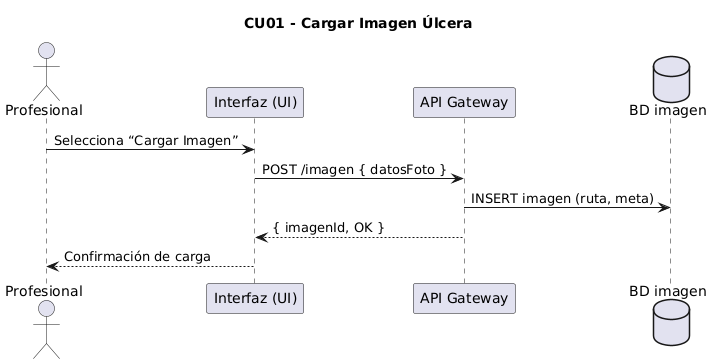
\includegraphics[width=0.8\textwidth]{imagenes/cu01_seq.png}
  \caption{CU01 – Cargar Imagen Úlcera. El Profesional sube o captura la fotografía clínica y el sistema la persiste en la base de datos de imágenes.}
  \label{fig:cu01_seq}
\end{figure}

\begin{figure}[H]
  \centering
  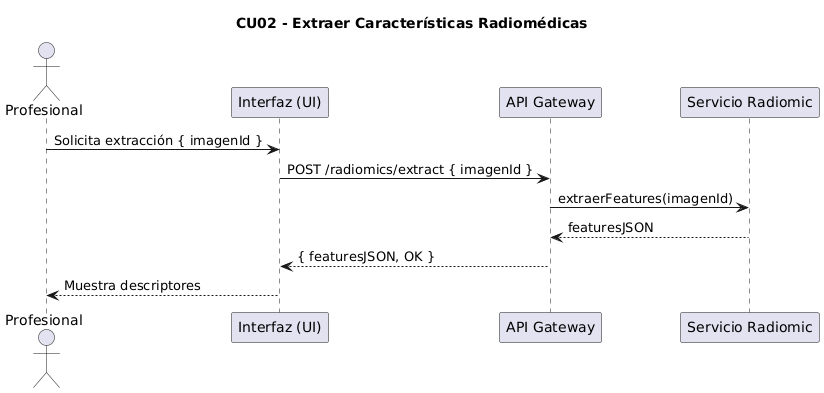
\includegraphics[width=0.8\textwidth]{imagenes/cu02_seq.png}
  \caption{CU02 – Extraer Características Radiomédicas. Después de la carga, el Profesional solicita el cálculo de descriptores radiómicos y el servicio asociado retorna los resultados.}
  \label{fig:cu02_seq}
\end{figure}

\begin{figure}[H]
  \centering
  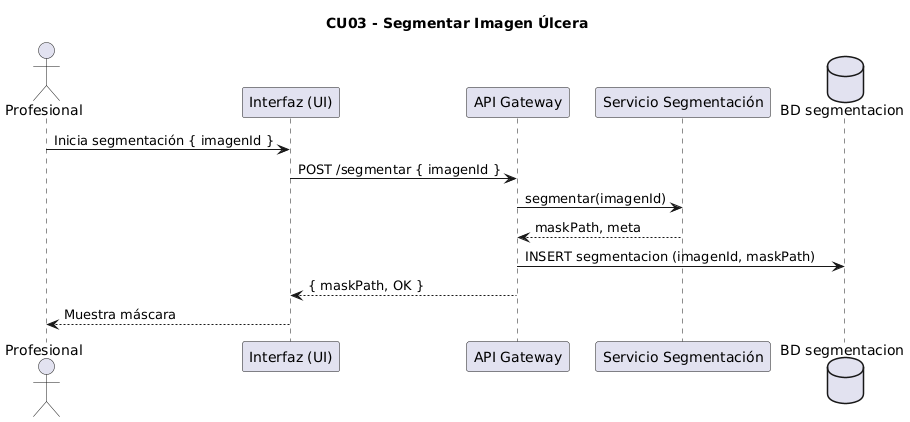
\includegraphics[width=0.8\textwidth]{imagenes/cu03_seq.png}
  \caption{CU03 – Segmentar Imagen Úlcera. El Profesional invoca la segmentación automática, que produce la(s) máscara(s) de herida y tejidos.}
  \label{fig:cu03_seq}
\end{figure}

\begin{figure}[H]
  \centering
  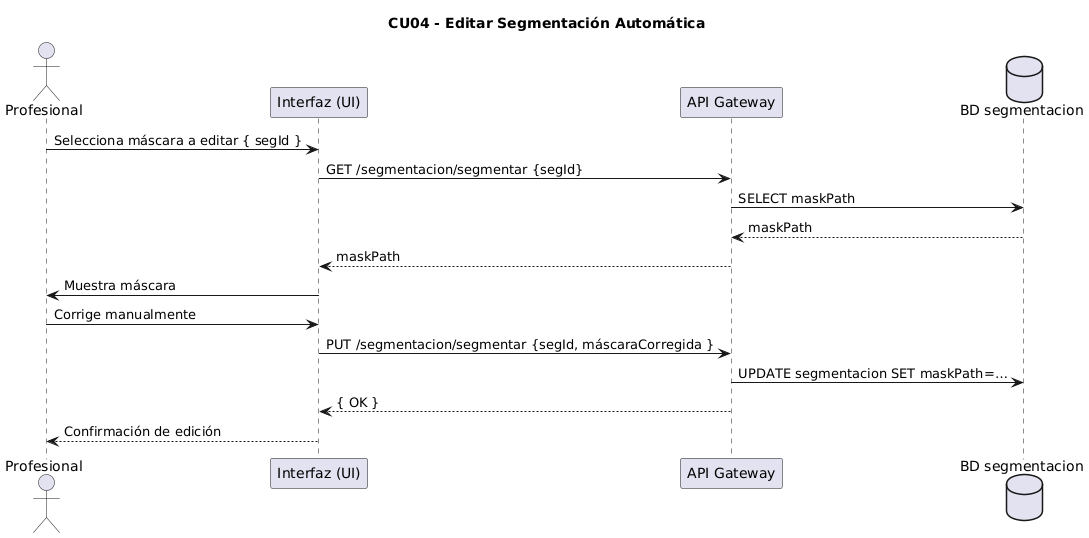
\includegraphics[width=0.8\textwidth]{imagenes/cu04_seq.png}
  \caption{CU04 – Editar Segmentación Automática. El Profesional corrige manualmente la máscara generada y almacena la versión ajustada.}
  \label{fig:cu04_seq}
\end{figure}

\begin{figure}[H]
  \centering
  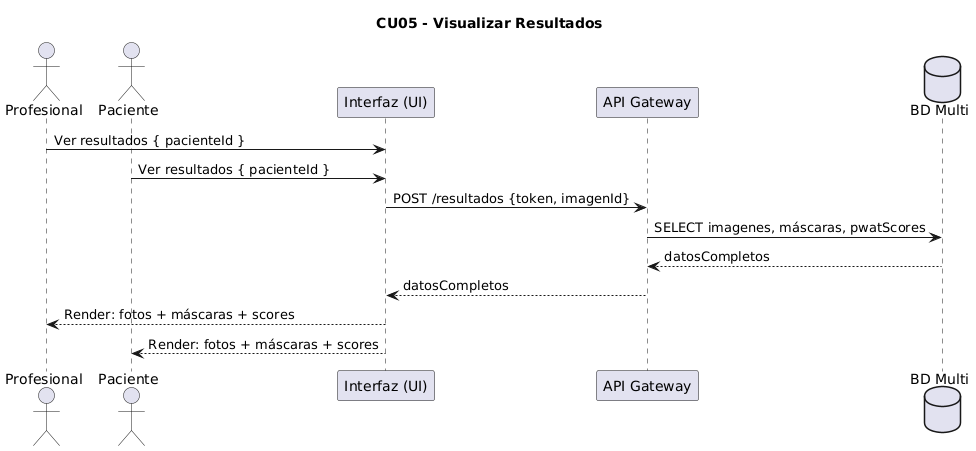
\includegraphics[width=0.8\textwidth]{imagenes/cu05_seq.png}
  \caption{CU05 – Visualizar Resultados. Profesional o Paciente recuperan y muestran la imagen, las máscaras y los puntajes PWAT generados.}
  \label{fig:cu05_seq}
\end{figure}

\begin{figure}[H]
  \centering
  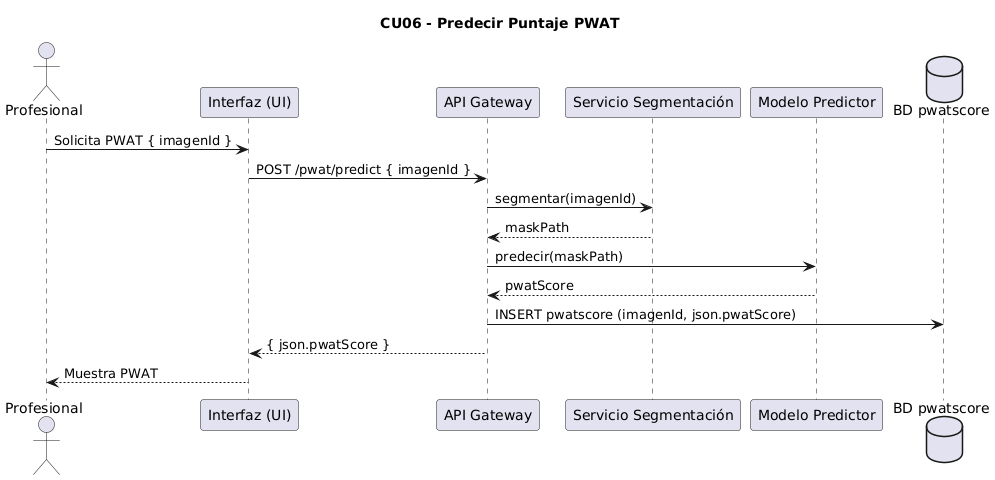
\includegraphics[width=0.8\textwidth]{imagenes/cu06_seq.png}
  \caption{CU06 – Predecir Puntaje PWAT. El Profesional solicita la predicción, se segmenta internamente y el Modelo Predictor devuelve el puntaje, que se guarda en la BD.}
  \label{fig:cu06_seq}
\end{figure}

\begin{figure}[H]
  \centering
  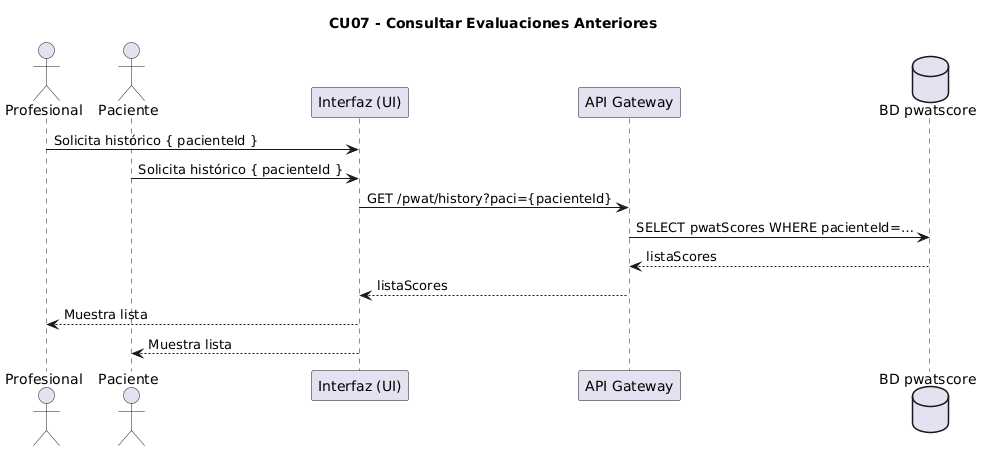
\includegraphics[width=0.8\textwidth]{imagenes/cu07_seq.png}
  \caption{CU07 – Consultar Evaluaciones Anteriores. Profesional o Paciente consultan el histórico de puntajes PWAT filtrados por paciente o imagen.}
  \label{fig:cu07_seq}
\end{figure}

\begin{figure}[H]
  \centering
  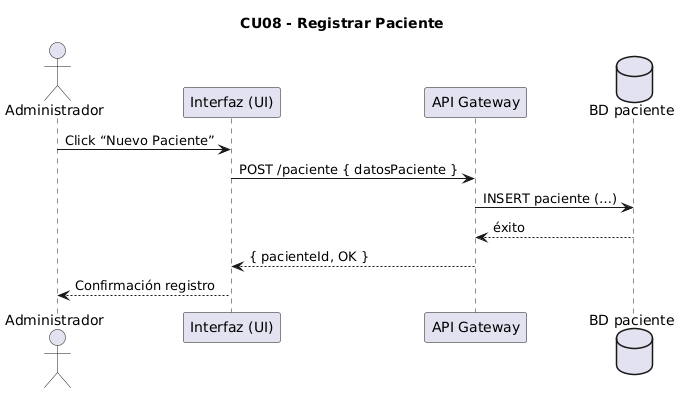
\includegraphics[width=0.8\textwidth]{imagenes/cu08_seq.png}
  \caption{CU08 – Registrar Paciente. El Administrador crea o actualiza registros en la tabla \texttt{paciente} mediante la interfaz.}
  \label{fig:cu08_seq}
\end{figure}

\begin{figure}[H]
  \centering
  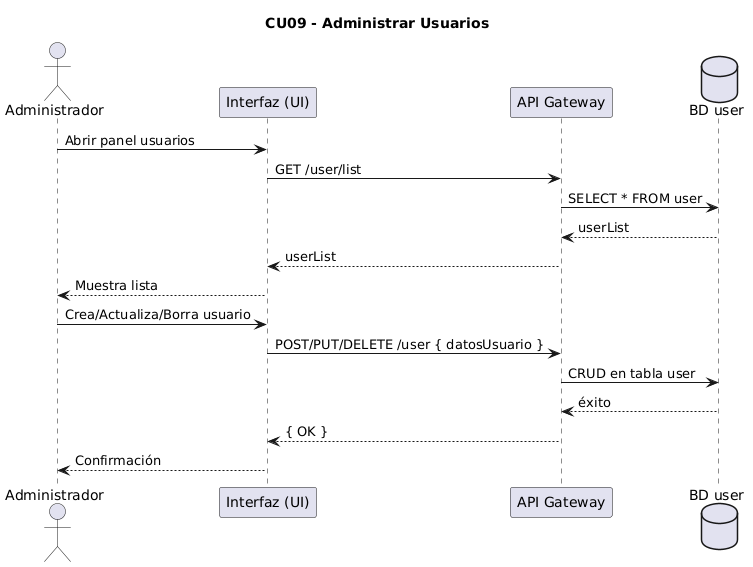
\includegraphics[width=0.8\textwidth]{imagenes/cu09_seq.png}
  \caption{CU09 – Administrar Usuarios. El Administrador realiza operaciones CRUD sobre la tabla \texttt{user}.}
  \label{fig:cu09_seq}
\end{figure}

\begin{figure}[H]
  \centering
  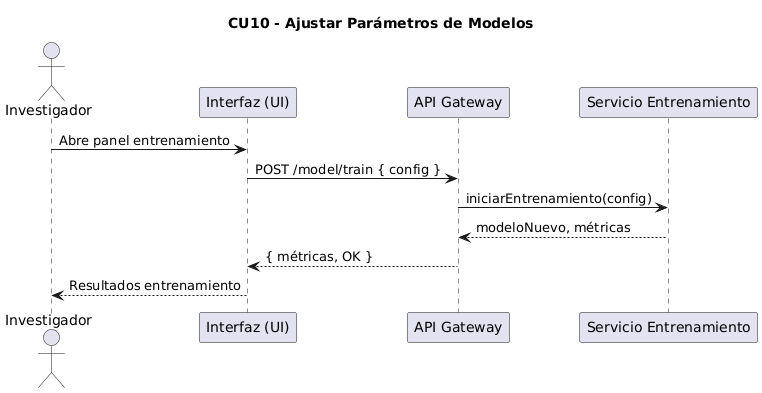
\includegraphics[width=0.8\textwidth]{imagenes/cu10_seq.png}
  \caption{CU10 – Ajustar Parámetros de Modelos. El Investigador lanza un nuevo entrenamiento o ajuste de hiperparámetros y recibe métricas.}
  \label{fig:cu10_seq}
\end{figure}

\begin{figure}[H]
  \centering
  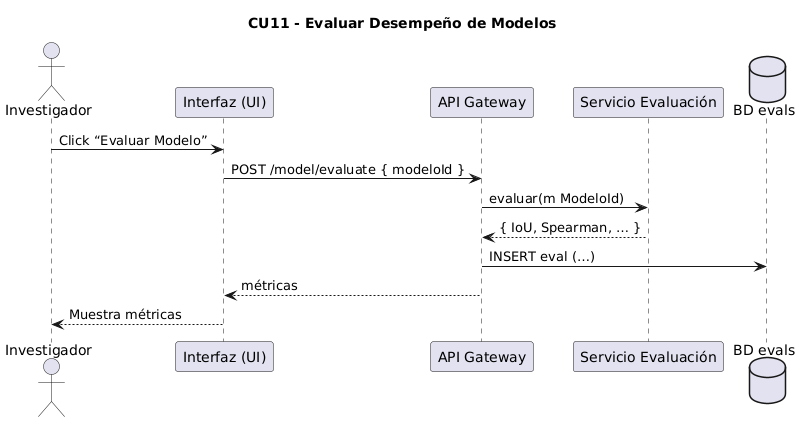
\includegraphics[width=0.8\textwidth]{imagenes/cu11_seq.png}
  \caption{CU11 – Evaluar Desempeño de Modelos. El Investigador solicita evaluación sobre test‐set y el sistema retorna métricas (IoU, Spearman, etc.).}
  \label{fig:cu11_seq}
\end{figure}

\subsection{Diagramas de Estado}
\label{ssc:DE}

A continuación se presentan los diagramas de estado para los tres elementos clave del sistema: \texttt{Imagen}, \texttt{Segmentación} y \texttt{PwatScore}. Cada figura muestra los estados por los que atraviesa el objeto y las transiciones disparadas por los casos de uso correspondientes.

\begin{figure}[H]
  \centering
  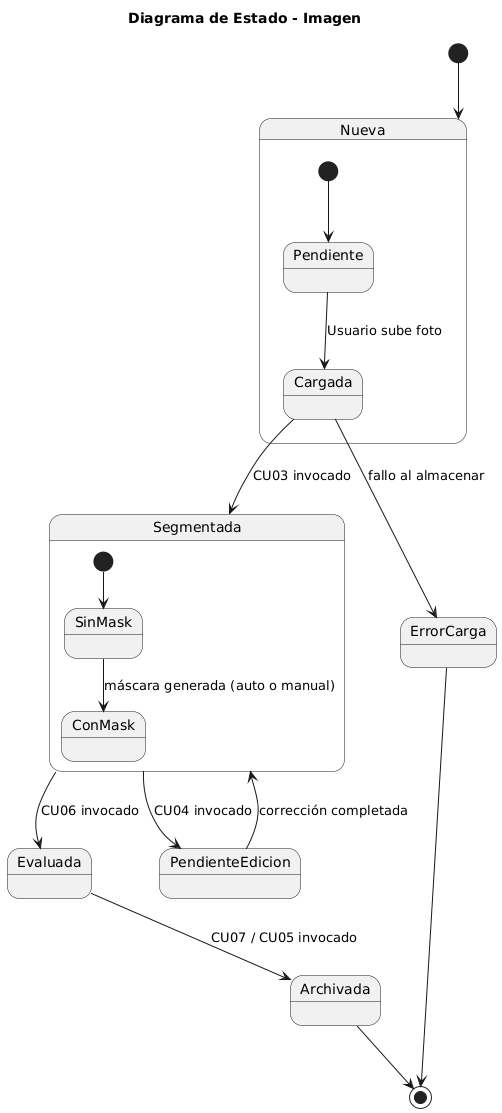
\includegraphics[width=0.95\textwidth,height=0.5\textheight,keepaspectratio]{imagenes/estado_imagen.png}
  \caption{Diagrama de estado de la entidad \texttt{Imagen}.}
  \label{fig:estado_imagen}
\end{figure}

\begin{figure}[H]
  \centering
  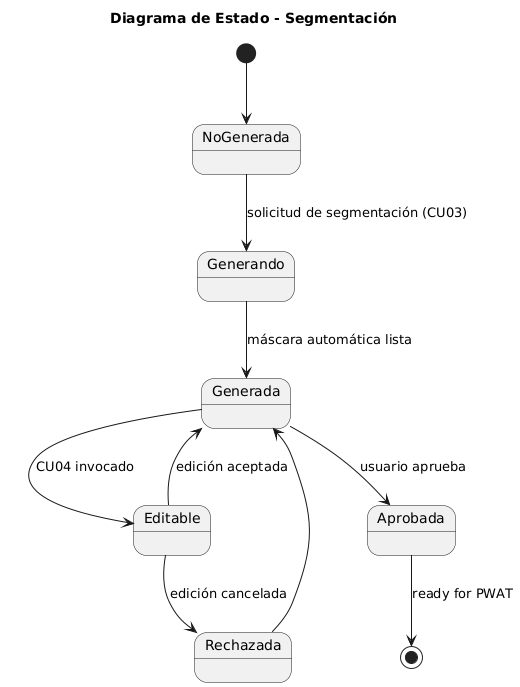
\includegraphics[width=0.95\textwidth,height=0.5\textheight,keepaspectratio]{imagenes/estado_segmentacion.png}
  \caption{Diagrama de estado de la entidad \texttt{Segmentación}.}
  \label{fig:estado_segmentacion}
\end{figure}

\begin{figure}[H]
  \centering
  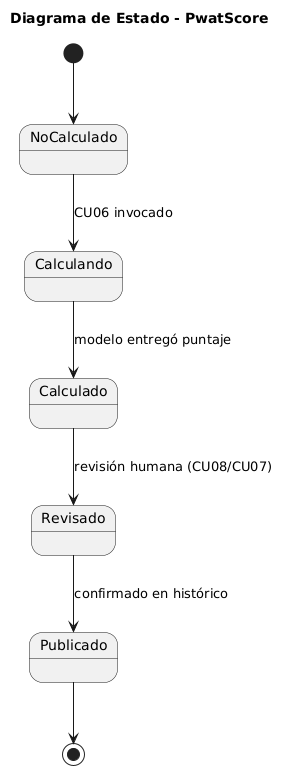
\includegraphics[width=0.95\textwidth,height=0.5\textheight,keepaspectratio]{imagenes/estado_pwatscore.png}
  \caption{Diagrama de estado de la entidad \texttt{PwatScore}.}
  \label{fig:estado_pwatscore}
\end{figure}

\subsection{Modelo Conceptual}
\label{ssc:MC}

A continuación se describe el modelo conceptual (diagrama de entidades y relaciones) que organiza las principales entidades del sistema y sus interacciones:

\begin{itemize}
  \item \textbf{User}: representa a todos los usuarios de la plataforma (clínicos, administradores e investigadores). Contiene atributos de identificación, datos de contacto y rol.
  \item \textbf{Profesional}: extiende a \texttt{User} con la especialidad y vincula al médico o enfermero responsable de pacientes.
  \item \textbf{Paciente}: almacena la información demográfica y clínica básica, referenciando al \texttt{User} que lo registró y al \texttt{Profesional} asignado.
  \item \textbf{Imagen}: guarda cada fotografía de la úlcera (nombre, fecha, ruta) asociada a un \texttt{Paciente}.
  \item \textbf{Segmentación}: registra cada máscara (método, ruta, fecha) aplicada sobre una \texttt{Imagen}, ya sea manual o automática.
  \item \textbf{PWATScore}: conserva los puntajes PWAT (valor numérico, evaluador, detalles en JSON, fecha), referenciando tanto la \texttt{Imagen} como la \texttt{Segmentación} empleada.
\end{itemize}

Las relaciones principales son:
\begin{itemize}
  \item Un \texttt{User} puede registrar múltiples \texttt{Profesional} y \texttt{Paciente}.
  \item Un \texttt{Profesional} está a cargo de cero o más \texttt{Paciente}.
  \item Cada \texttt{Paciente} puede tener varias \texttt{Imagen}, y cada \texttt{Imagen} puede generar múltiples \texttt{Segmentación} y \texttt{PWATScore}.
  \item Cada \texttt{Segmentación} está vinculada a una única \texttt{Imagen}, y cada \texttt{PWATScore} se apoya en una \texttt{Imagen} y una \texttt{Segmentación}.
\end{itemize}

Este esquema asegura la trazabilidad completa desde el registro de usuarios y pacientes, pasando por la captura y segmentación de imágenes, hasta la evaluación cuantitativa del estadio de la herida mediante puntajes PWAT.

\begin{figure}[H]
  \centering
  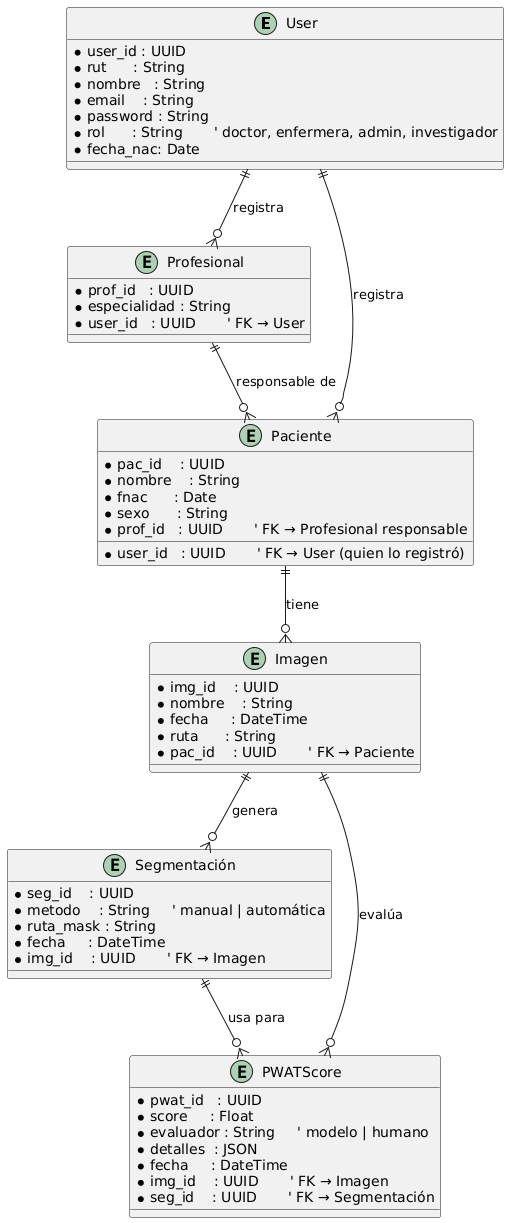
\includegraphics[
    width=\textwidth,
    height=0.9\textheight,
    keepaspectratio
  ]{imagenes/modelo_conceptual.png}
  \caption{Diagrama conceptual de entidades y relaciones del sistema.}
  \label{fig:modelo_conceptual}
\end{figure}


\chapter{Diseño}
\label{ch:Impl}    
\section{Diseño Arquitectónico}
\label{sc:DA}

\subsection{Tecnologías utilizadas}
\label{ssc:tech}

El sistema se compone de tres módulos principales, cada uno encargado de una función especifica dentro del flujo de análisis de ulceras.
\subsection{Backend}
\begin{description}
    \item[Función] Exponer un conjunto de servicios REST para gestionar usuarios, pacientes, imágenes y segmentaciones. 
    \item[Persistencia] Un ORM sobre MySQL facilita la definición de las entidades de dominio y sus relaciones 
    \item[Seguridad] Autentificación mediante tokens, junto con un mecanismo de hashing para las credenciales.
    \item[Manejo de archivos] Recepción, almacenamiento y registro de imágenes y mascaras de segmentación.
    \item[Integración con el modelo de ML] Invoca de forma transparente la lógica de análisis y segmentación desarrollada en Python   
\end{description}

\subsection{Frontend}
\begin{description}
\item[Función] Ofrecer una interfaz web para autenticación, visualización de pacientes y gestión de resultados.
\item[Rendimiento y experiencia] Renderizado inicial en servidor y enrutamiento automático para mejorar tiempos de carga y SEO.
\item[Comunicación] Consumo de los servicios del backend, adjuntando el token de autenticación en cada solicitud.
\item[Componentes] Elementos reutilizables para formularios de acceso, panel de imágenes y tablas de datos.
\end{description}

\subsection{Categorizador}
\begin{description}
\item[Función] Ejecución de algoritmos de visión por computador y machine learning para segmentar imágenes y calcular puntajes clínicos.
\item[Tecnologías] Bibliotecas especializadas en procesamiento de imágenes y aprendizaje automático.
\item[Modo de operación]
\begin{itemize}
\item Segmentación de la zona lesionada.
\item Evaluación y asignación de un puntaje en la escala PWAT.
\end{itemize}
\item[Salida] Máscaras segmentadas y valores de puntuación, disponibles para su consulta en el sistema.
\end{description}

\subsection{Visión Unificada}
Este enfoque modular garantiza:
\begin{itemize}
\item Desarrollo y despliegue independientes por componente.
\item Mantenibilidad y escalabilidad a medida que evolucionan los requerimientos.
\item Aprovechamiento de cada tecnología en su área de fortaleza: servicios web, interfaces dinámicas y modelos de inteligencia artificial.
\end{itemize}



\subsection{Flujo de datos / Vista de alto nivel}
\label{ssc:flow}

Para comprender el funcionamiento global de la plataforma, se describira el recorrido que sigue la información desde el momento en que el usuario inicia una acción hasta que obtiene el resultado final. Esta visión de alto nivel permite apreciar de forma clara y ordenada los componentes implicados y la secuencia de procesos que garantizan el correcto manejo de imágenes, metadatos y resultados de segmentación.

En primer lugar, el usuario interactúa mediante la interfaz web, donde sus solicitudes (por ejemplo, carga de imágenes o consulta de resultados previos) son capturadas y enviadas al servidor. A continuación, el módulo de frontend traduce estas peticiones a llamadas a la API REST, incorporando el token de autenticación para validar el acceso. 

El backend recibe la petición, valida los datos y coordina dos tareas principales:  
\begin{enumerate}
  \item \emph{Persistencia}: guarda o recupera los datos relevantes (tipo de usuario: paciente, imágenes, máscaras) en la base de datos.
  \item \emph{Análisis}: cuando se solicita segmentación o cálculo de puntaje, despacha la petición al módulo de categorización, ejecutando el proceso de visión por computador y machine learning en Python.
\end{enumerate}

El módulo de categorizador procesa la imagen, genera la máscara de la lesión y calcula el puntaje clínico, devolviendo estos resultados al backend. Finalmente, el backend almacena la nueva información y responde al frontend con los datos actualizados, que se presentan al usuario mediante componentes interactivos.  

De este modo, el flujo de datos se organiza en cuatro fases —recolección, procesamiento, persistencia y visualización—, garantizando un tránsito de información seguro, escalable y transparente para el investigador o profesional clínico que utilice la plataforma. La Figura \ref{fig:arquitectura-alto-nivel} ilustra estos pasos en un diagrama de alto nivel.  

\begin{figure}[H]
  \centering
  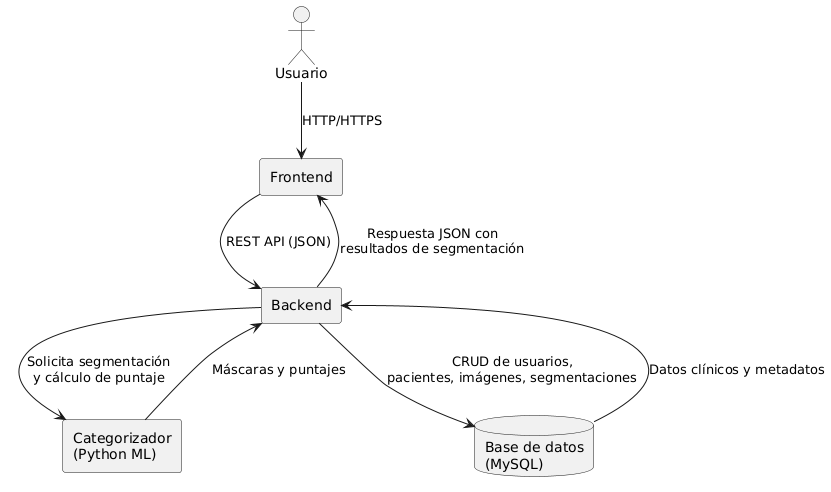
\includegraphics[width=0.8\textwidth,height=0.5\textheight,keepaspectratio]{imagenes/esquemaAlto.png}
  \caption{Esquema de alto nivel del sistema.}
  \label{fig:arquitectura-alto-nivel}
\end{figure}


\subsection{Diagrama de despliegue}
\label{ssc:diagDesp}

\subsubsection{Cliente Web}
Este nodo representa el navegador del usuario, donde se ejecuta la aplicación SPA \footnote{SPA: Single Page Application, es un tipo de aplicación web que se carga una sola vez en el navegador y luego interactúa con el usuario actualizando dinámicamente el contenido de la página sin necesidad de recargarla por completo} construida con Next.js y React. Depende de los artefactos estáticos generados (HTML, CSS y JavaScript) agrupados en un paquete de frontend. La comunicación se realiza sobre HTTP/HTTPS hacia el servidor de la aplicación, enviando solicitudes de carga de imágenes, autentificación y recuperación de datos. Al existir rutas automáticas y rende rizado inicial en servidor, el cliente recibe primero HTML pre-renderizado y luego gestiona de forma reactiva las interacciones con la interfaz

\subsubsection{Servidor de Aplicación}
Agrupa dos paquetes lógicos: el frontend de Next.js y el backend de Express. El paquete de frontend sirve los ficheros estáticos y gestionará el SSR; el de backend expone una API REST para CRUD de usuarios, imágenes y segmentaciones. Internamente, ambos comparten dependencias de Node.js y se despliegan como un mismo contenedor o instancia, garantizando coherencia entre presentación y lógica de negocio. El backend recibe peticiones JSON del cliente, valida tokens y enruta las operaciones según la capa de persistencia o la de análisis.

\subsubsection{Servidor de ML (Categorizador)}
Aislado en una máquina que ejecuta un entorno Python con bibliotecas de visión por computador (OpenCV, PIL, pyradiomics) y aprendizaje automático (scikit-learn, XGBoost, TensorFlow/Keras). Depende de un entorno gestionado por \texttt{Conda} que agrupa todos los módulos necesarios. La interacción con el servidor de aplicación es síncrona: este último envía la imagen a procesar y recibe de vuelta la máscara segmentada y el puntaje PWAT en formato JSON o archivos. De este modo, la lógica de machine learning permanece desacoplada de Node.js.

\subsubsection{Servidor de Base de Datos}
Un servicio MySQL que persiste toda la información clínica y metadatos de imágenes, máscaras y resultados. El backend utiliza un ORM (Sequelize) y el driver mysql2 para comunicarse con este nodo, ejecutando operaciones CRUD. La conexión viaja por la red interna usando el protocolo MySQL; así se separa la capa de datos de las capas de aplicación y análisis, permitiendo escalado independiente y facilidades de respaldo.

\begin{figure}[H]
    \centering
    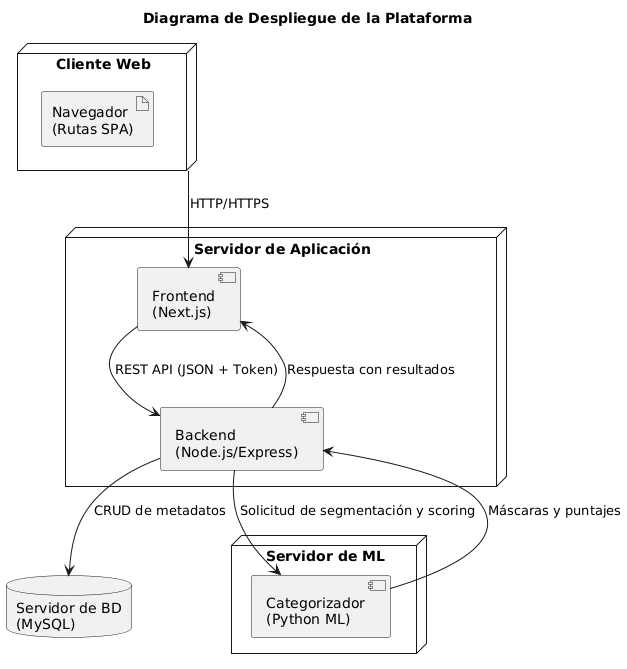
\includegraphics[width=0.8\textwidth,height=0.5\textheight,keepaspectratio]{imagenes/despliegue.png}
    \caption{Diagrama de Despliegue}
    \label{fig:DD}
\end{figure}


\subsection{Diagrama de componentes}
\label{ssc:diaComp}

A continuacion se presenta el diagrama de componentes que sintetiza la organización modular de la plataforma. En el se identifican las unidades lógicas (Frontend, Backend, Categorizador y sistemas de almacenamiento) y los contratos de servicio (interfaces) que establecen sus puntos de interacción. Esta representación y el flujo de dependencias entre los distintos subsistemas.


\begin{figure}[H]
    \centering
    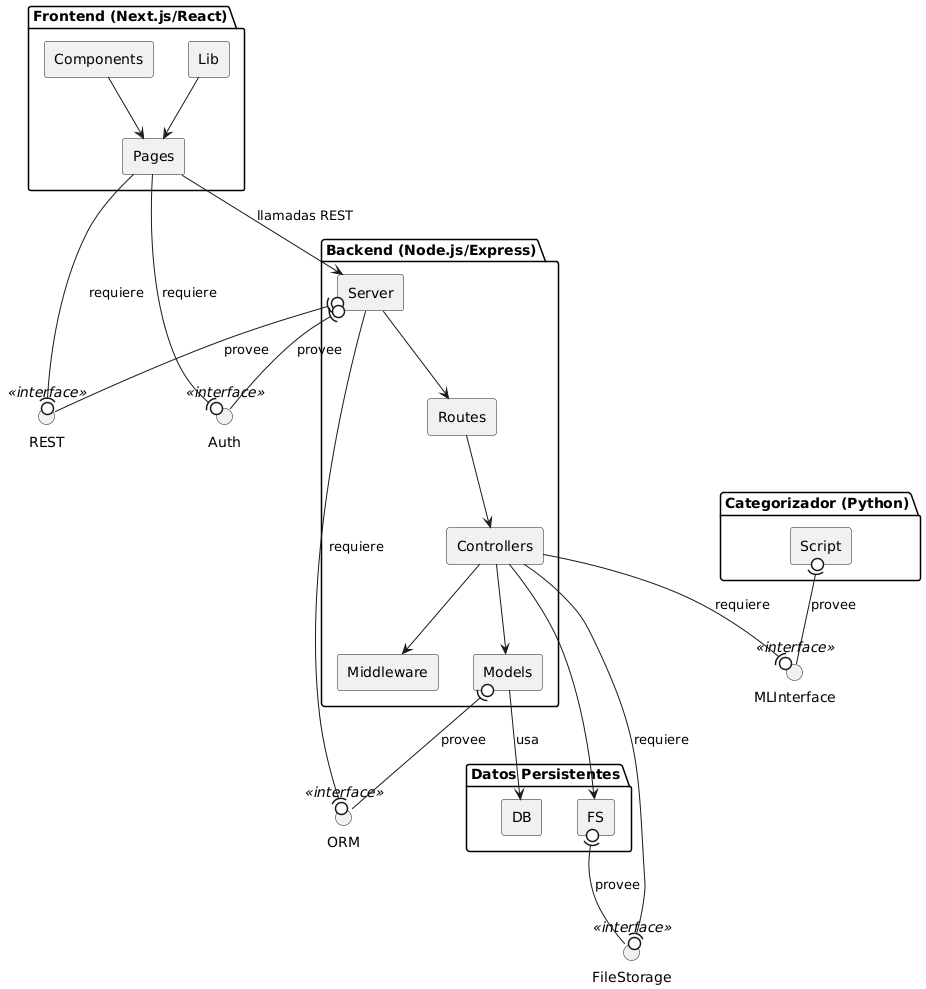
\includegraphics[width=0.7\linewidth]{imagenes/componentes.png}
    \caption{Diagrama de Componentes}
    \label{fig:componentDiagram}
\end{figure}
    
    
    
\subsection{Diagrama de paquetes}
\label{ssc:pack}
    
A continuación se presenta el diagrama de paquetes que ofrece una visión de alto nivel de la estructura modular del sistema. Cada recuadro agrupa elementos relacionados —páginas, componentes, utilidades y estilos del frontend; configuración, middleware, modelos, controladores y rutas del backend; el script de categorización en Python; y los elementos de persistencia de datos— mostrando cómo se organizan y encapsulan las responsabilidades. Las flechas con estereotipos (\texttt{<<uses>>}, \texttt{<<import>>}, \texttt{<<access>>}) indican las dependencias principales entre paquetes: el frontend consume servicios REST del backend, éste orquesta modelos y controladores y lanza el script de PWAT, y finalmente los módulos acceden a la base de datos y al sistema de archivos para leer o almacenar información. Este esquema facilita entender, de un vistazo, qué agrupa cada paquete y cómo fluye la comunicación entre ellos antes de profundizar en los detalles de implementación.

\begin{figure}[H]
    \centering
    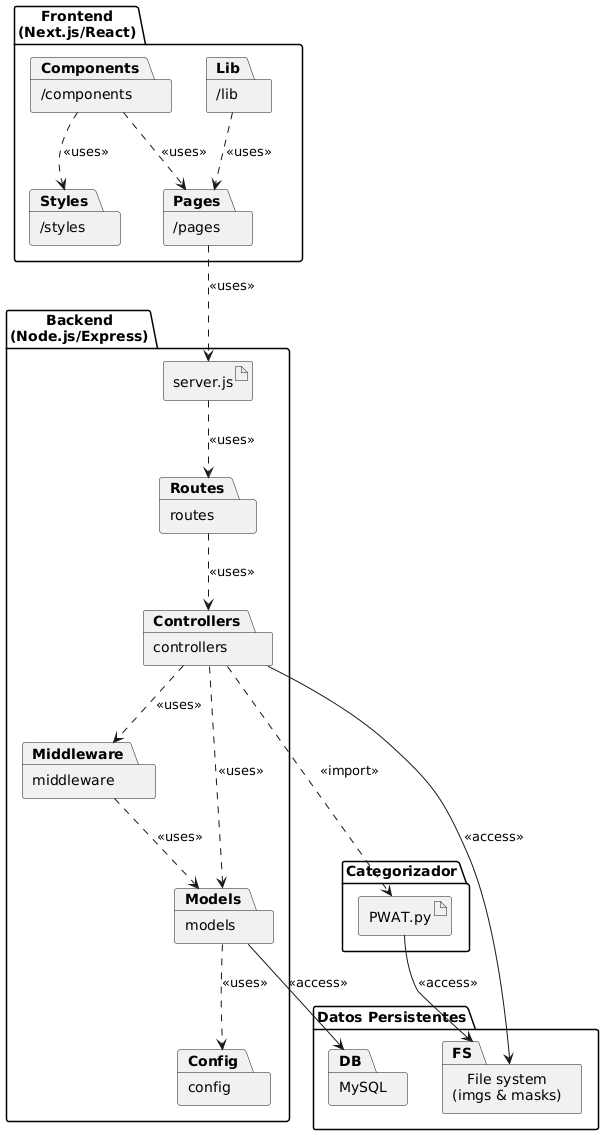
\includegraphics[width=0.7\linewidth]{imagenes/paquetes.png}
    \caption{Diagrama de Paquetes}
    \label{fig:packageDiagram}
\end{figure}
    
\subsection{Diagrama de clases}
\label{ssc:clases}
A continuación se muestra el diagrama de clases que describe el modelo de dominio central de la plataforma. En él aparecen:
Las entidades de gestión de usuarios:
\begin{itemize}
    \item  User
    \item Profesional
    \item Paciente
\end{itemize}
Con sus todos atributos y operaciones principales.

El paquete de contenido clínico
\begin{itemize}
    \item Imagen
    \item Segmentacion
    \item PWATScore
\end{itemize}

Estos modelan la captura, tratamiento y evaluacion de las heridas

Las relaciones y cardinalidades revelan cómo un usuario se vincula a un profesional o paciente, cómo un paciente puede tener múltiples imágenes, y cómo cada imagen da lugar a múltiples segmentaciones y puntuaciones.
Este esquema estático ofrece una visión clara de las piezas independientes del sistema y sus conexiones, sirviendo como referencia para el desarrollo, la integración y la evolución de la plataforma.
\begin{figure}[H]
  \centering
  \adjustbox{%
    max width=\textwidth,       % como mucho el ancho del texto
    max height=1.3\textheight,   % o el 90% de la altura del área imprimible
    keepaspectratio             % sin deformar
  }{%
    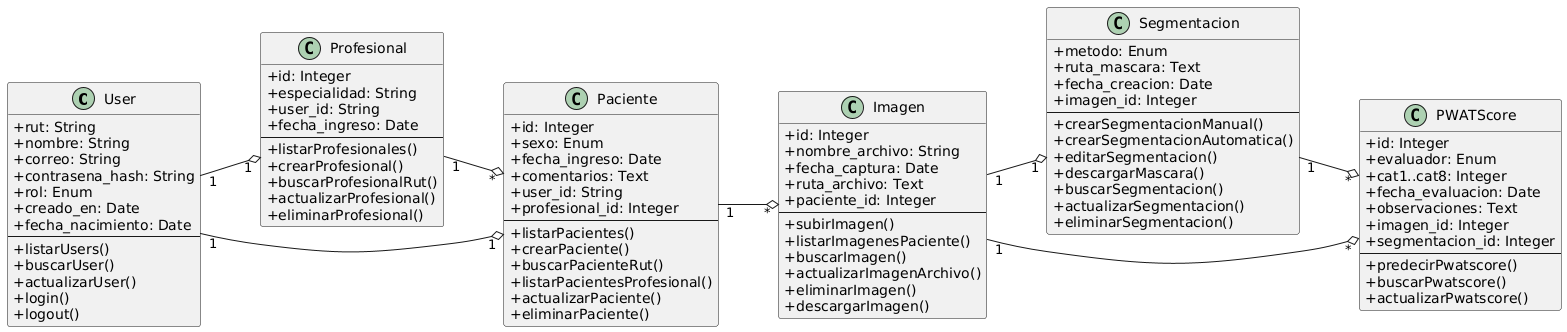
\includegraphics{imagenes/clases.png}%
  }
  \caption{Modelo Relacional}
  \label{fig:classesDiagram}
\end{figure}


\section{Diseño de Datos}
\label{sc:DD}

\subsection{Diagrama Entidad Relación}
\label{ssc:ER}
A continuación se presenta el diagrama entidad-relación en notación de Chen \cite{chen1976entity} que sintetiza la estructura lógica de la base de datos. En él se identifican las seis entidades principales (User, Profesional, Paciente, Imagen, Segmentación y PWATScore), sus atributos clave y las relaciones que las vinculan (EsPaciente, EsProfesional, Atiende, Posee, Genera, Evalua y Deriva), con sus cardinalidades asociadas. Este modelo de alto nivel facilita la comprensión del esquema de almacenamiento de datos antes de pasar a detalles de implementación.
\begin{figure}[H]
    \centering
    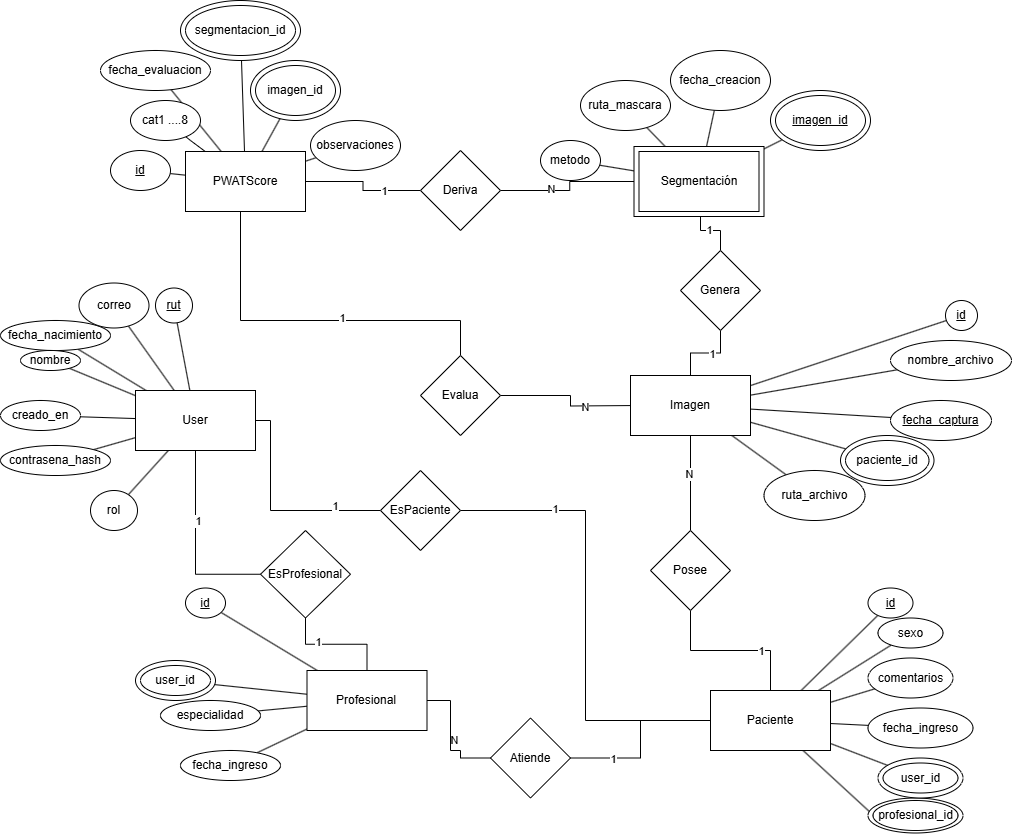
\includegraphics[width=1\linewidth]{imagenes/ER (1).png}
    \caption{Diagrama Entidad Relacion}
    \label{fig:classesDiagram}
\end{figure}

\subsection{Modelo Relacional}
\label{ssc:Rel}

A continuación se presenta el modelo relacional que refleja la implementación en MySQL de las entidades y relaciones definidas en el esquema ER. Cada rectángulo representa una tabla con sus columnas y restricciones principales (PK, FK, UQ), mientras que las líneas indican las relaciones entre tablas con sus cardinalidades (1:1, 1:N). Este diagrama facilita la lectura de la estructura de la base de datos y sirve de guía para generar las sentencias DDL\footnote{DDL: Data Definition Language o Lenguaje de Definicion de Datos.} correspondientes.
\begin{figure}[H]
  \centering
  \adjustbox{%
    max width=\textwidth,       % como mucho el ancho del texto
    max height=0.70\textheight,   % o el 90% de la altura del área imprimible
    keepaspectratio             % sin deformar
  }{%
    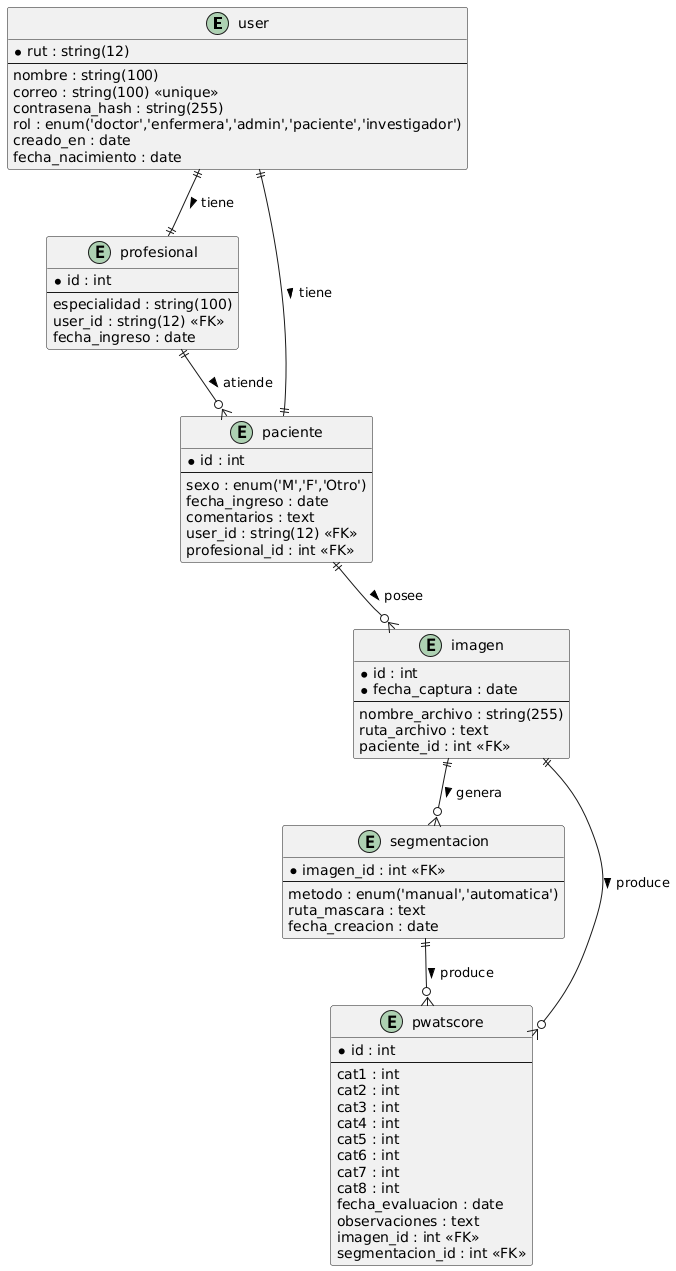
\includegraphics{imagenes/relacional.png}%
  }
  \caption{Modelo Relacional}
  \label{fig:classesDiagram}
\end{figure}



\subsection{Diccionario de Datos}
\label{ssc:DD}
A continuación se incluye el Diccionario de Datos de la base de datos relacional. En él se describen de forma detallada cada una de las tablas —con sus claves primarias, foráneas y restricciones de unicidad— así como los atributos que las componen, su tipo de datos y su significado dentro del sistema. Este artefacto sirve como referencia para el equipo de desarrollo y como documentación formal de la estructura de almacenamiento, facilitando la generación de los scripts DDL y garantizando la consistencia e integridad de la información durante todo el ciclo de vida del proyecto.

\renewcommand{\arraystretch}{1.0}   % Menos altura de fila

\subsection*{Tabla \texttt{User}}
{\footnotesize
\begin{tabularx}{\textwidth}{l l l X}
\hline
\textbf{Atributo} & \textbf{Tipo} & \textbf{Restricción} & \textbf{Descripción} \\\hline
rut               & VARCHAR(20)   & PK                   & RUT del usuario, único e identifica al usuario. \\
nombre            & VARCHAR(100)  & —                    & Nombre completo. \\
correo            & VARCHAR(150)  & UQ                   & Correo electrónico. \\
contrasena\_hash  & VARCHAR(255)  & —                    & Hash de la contraseña. \\
rol               & ENUM          & —                    & Perfil (\texttt{admin}, \texttt{profesional}, \texttt{paciente}). \\
creado\_en        & DATETIME      & —                    & Fecha de creación. \\
fecha\_nacimiento & DATE          & —                    & Fecha de nacimiento. \\\hline
\end{tabularx}
}

\subsection*{Tabla \texttt{Profesional}}
{\footnotesize
\begin{tabularx}{\textwidth}{l l l X}
\hline
\textbf{Atributo} & \textbf{Tipo}       & \textbf{Restricción} & \textbf{Descripción} \\\hline
id                & INT AUTO\_INCREMENT & PK                   & Identificador único. \\
user\_id          & VARCHAR(20)         & FK                   & RUT del usuario. \\
especialidad      & VARCHAR(100)        & —                    & Área de especialidad. \\
fecha\_ingreso    & DATE                & —                    & Fecha de alta. \\\hline
\end{tabularx}
}

\subsection*{Tabla \texttt{Paciente}}
{\footnotesize
\begin{tabularx}{\textwidth}{l l l X}
\hline
\textbf{Atributo} & \textbf{Tipo}              & \textbf{Restricción}  & \textbf{Descripción} \\\hline
id               & INT AUTO\_INCREMENT        & PK                    & Identificador del paciente. \\
sexo             & ENUM                       & —                     & Sexo biológico (\texttt{M}, \texttt{F}). \\
fecha\_ingreso   & DATE                       & —                     & Fecha de registro. \\
comentarios      & TEXT                       & —                     & Notas o comentarios. \\
user\_id         & VARCHAR(20)                & FK                    & RUT de usuario. \\
profesional\_id  & INT                        & FK                    & Profesional a cargo. \\\hline
\end{tabularx}
}

\subsection*{Tabla \texttt{Imagen}}
{\footnotesize
\begin{tabularx}{\textwidth}{l l l X}
\hline
\textbf{Atributo} & \textbf{Tipo}            & \textbf{Restricción} & \textbf{Descripción} \\\hline
id               & INT AUTO\_INCREMENT      & PK                   & Identificador de imagen. \\
fecha\_captura   & DATETIME                 & PK                   & Marca temporal. \\
nombre\_archivo  & VARCHAR(200)             & —                    & Nombre de fichero. \\
ruta\_archivo    & TEXT                     & —                    & Ruta en disco. \\
paciente\_id     & INT                      & FK                   & Paciente asociado. \\\hline
\end{tabularx}
}

\subsection*{Tabla \texttt{Segmentacion}}
{\footnotesize
\begin{tabularx}{\textwidth}{l l l X}
\hline
\textbf{Atributo} & \textbf{Tipo}            & \textbf{Restricción} & \textbf{Descripción} \\\hline
metodo           & ENUM                      & —                    & Tipo (\texttt{manual}, \texttt{automatica}). \\
ruta\_mascara    & TEXT                     & —                    & Ruta de la máscara. \\
fecha\_creacion  & DATETIME                 & —                    & Fecha de creación. \\
imagen\_id       & INT                      & FK PK                  & Imagen asociada. \\\hline
\end{tabularx}
}

\subsection*{Tabla \texttt{PWATScore}}
{\footnotesize
\begin{tabularx}{\textwidth}{l l l X}
\hline
\textbf{Atributo}      & \textbf{Tipo}         & \textbf{Restricción} & \textbf{Descripción} \\\hline
id                    & INT AUTO\_INCREMENT   & PK                   & ID del registro. \\
cat1–cat8             & INT                   & —                    & Categorías clínicas (1–8). \\
fecha\_evaluacion     & DATETIME              & —                    & Fecha de evaluación. \\
observaciones         & TEXT                  & —                    & Comentarios adicionales. \\
imagen\_id            & INT                   & FK                   & Imagen evaluada. \\
segmentacion\_id      & INT                   & FK                   & Segmentación usada. \\\hline
\end{tabularx}
}

\subsection{Diagrama de Flujo de datos}

A continuación se describe el recorrido de la información a través de los distintos módulos de la plataforma:

\begin{enumerate}
  \item \textbf{Interacción de usuario y Frontend}  
    Los componentes de la interfaz (botones, formularios, listados) y las páginas de Next.js reciben las acciones del usuario (por ejemplo, carga de imagen o petición de historial). Estas páginas utilizan el helper de API (\texttt{api.js}) para generar peticiones REST al servidor, adjuntando el token JWT para autorizar cada solicitud.
  
  \item \textbf{Procesamiento en el Backend}  
    El servidor Express recibe cada solicitud y la enruta según su endpoint. A través de las capas de rutas y controladores se valida la entrada, se gestionan credenciales y se aplican reglas de negocio. Los controladores interactúan con los modelos Sequelize para leer o escribir datos en la base de datos MySQL.
  
  \item \textbf{Gestión de archivos y análisis}  
    Cuando corresponde, los controladores también almacenan o recuperan imágenes y máscaras en el sistema de archivos. Para la segmentación automática y el cálculo del PWATScore, el backend invoca de forma asíncrona el script de Python (\texttt{PWAT.py}), pasando la ruta del archivo. El script procesa la imagen, genera las máscaras y devuelve los resultados, que se guardan nuevamente en disco.
  
  \item \textbf{Respuesta al Frontend}  
    Una vez completado el procesamiento —persistencia en la base de datos, almacenamiento de archivos y análisis de ML— el backend construye la respuesta JSON con los datos solicitados (por ejemplo, URLs de las máscaras, valores de puntaje). El frontend recibe estos datos y los muestra en la interfaz, ofreciendo al usuario un feedback inmediato y la posibilidad de seguir navegando o realizar nuevas acciones.
\end{enumerate}

\begin{figure}[H]
    \centering
    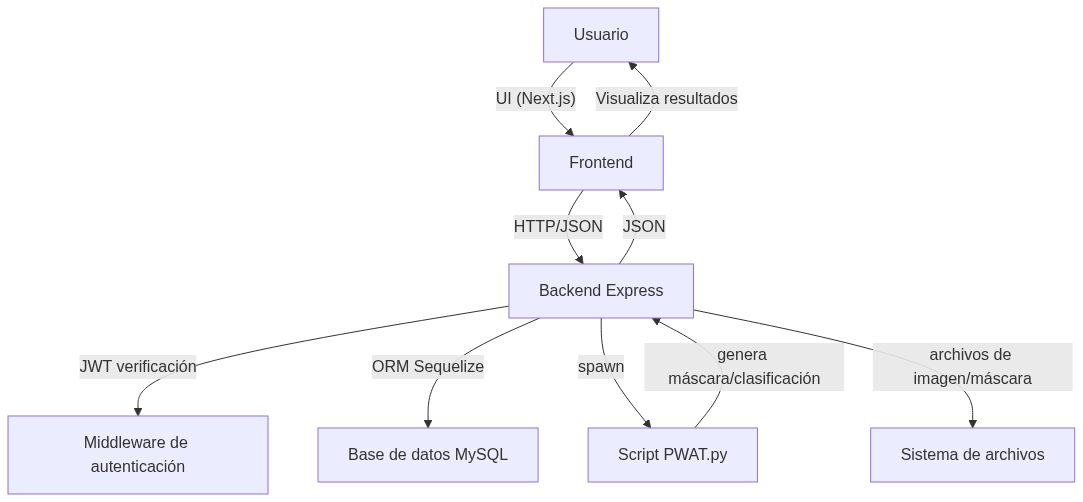
\includegraphics[width=1\linewidth]{imagenes/flujo.png}
    \caption{Modelo Relacional}
    \label{fig:classesDiagram}
\end{figure}

\section{Diseño de Interfaz}
\label{sc:DI}

Para prensetar el alcance de la aplicaciom de gestion y revision de imagenes, se empleo un esquema de interfaces de alto nivel, mostrando a su alrededor los cuatro actores principales: \textbf{Administrador}, \textbf{Profesional}, \textbf{Investigador} y \textbf{Paciente}. Cada uno de ellos interactua con el interfaz web (implementada en React/Next.js) para realizar su funcionalidad especifica: el \textbf{Administrador} gestiona usuarios y asignaciones, el \textbf{Investigador} consulta metricas y lanza procesos de rentremamiento, el \textbf{Profesional} lista pacientes y sube o reemplaza imagenes, y el \textbf{Paciente} edita su perfil y revisa sus historiales.


\begin{figure}[H]
    \centering
    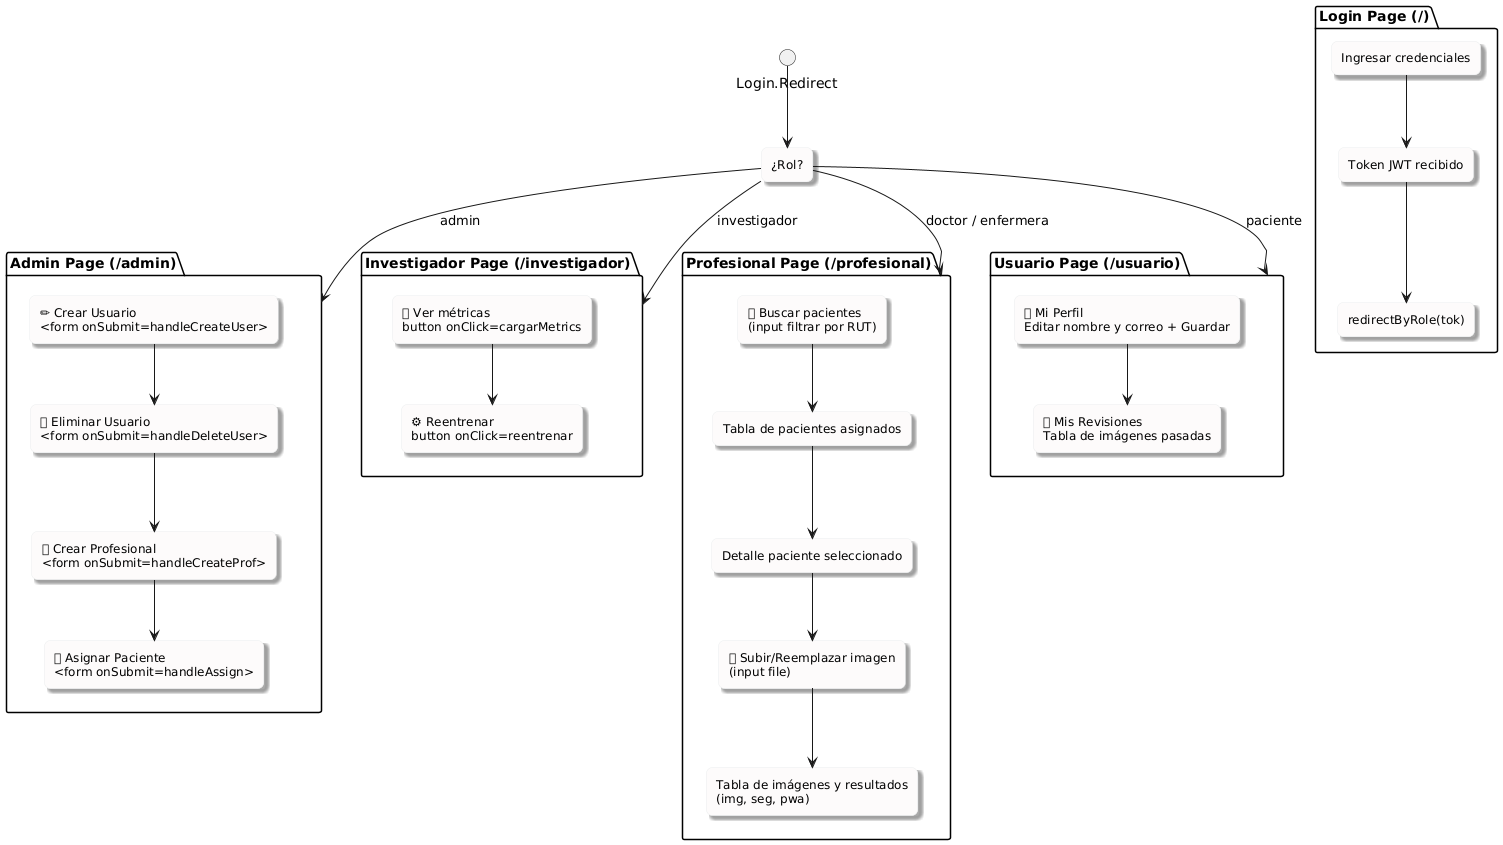
\includegraphics[width=1\linewidth]{imagenes/esquema.png}
    \caption{Modelo Relacional}
    \label{fig:classesDiagram}
\end{figure}


%\subsection{Prototipos de Interfaces Gráficas}
%\label{ssc:IGraph}


\section{Diseño de Pruebas}
\label{sc:DP}

Este plan de pruebas se estructura según los principales módulos del sistema: Backend (Node.js/Express), Frontend (Next.js) y Categorizador (Python). Cada componente tiene pruebas asociadas para asegurar su correcto funcionamiento, integración y robustez frente a errores

\subsubsection{Backend}
\textbf{Cobertura de pruebas}
\begin{itemize}
    \item Pruebas Unitarias:
    \begin{itemize}
        \item Cada controlador cuenta con pruebas especificas que verifiquen el comportamiento aislado de sus funciones principales
    \end{itemize}
\begin{itemize}
    \item Se utilizan herramientas como Supertest para simular el entorno de ejecución y mockear dependencias externas
    \item Conexión y operaciones en base de datos de pruebas o uso de mocks de Sequelize
    \item Validación de relaciones entre modelos y respuestas ante inconsistencias
\end{itemize}
\end{itemize}

\subsubsection{Frontend}
\textbf{Cobertura de pruebas}
\begin{itemize}
    \item Pruebas de componentes
    \begin{itemize}
        \item Validación de renderizado correcto y comportamiento de componentes
    \end{itemize}
\begin{itemize}
    \item Simulación de interacciones en formularios
\end{itemize}
\begin{itemize}
    \item Validación de que las peticiones incluyen correctamente los tokens de autenticación
    \item Flujo completo desde login hasta la evaluación de la ulcera
\end{itemize}
\end{itemize}
\subsubsection{Categorizador}
\textbf{Cobertura de pruebas}
\begin{itemize}
    \item Pruebas unitarias
    \begin{itemize}
        \item Escritura y lectura de archivos de imagen y mascaras
        \item Funciones como \texttt{predecir\_mascara}, \texttt{predecir} y \texttt{mask\_predict} se prueban de forma aislada
    \end{itemize}
\end{itemize}

\subsection{Pruebas Unitarias}
\label{ssc:UT}

\begin{enumerate}
    \item \textbf{Backend}
    \begin{enumerate}
        \item \texttt{User.crearUser} debe crear un nuevo usuario con datos validos
        \item \texttt{User.listarUsers} debe retornar todos los usuarios desde la base de datos
        \item \texttt{Pacientes.crearPaciente} debe validar datos requeridos y retornar error si falta
        \item \texttt{Segmentacion.crearSegmentacion} debe recibir la imagen y generar peticion al categorizador
        \item \texttt{PWATScore.calcularPWAT} debe devolver correctamente el puntaje basado en la mascara
    \end{enumerate}
\item \textbf{Frontend}
\begin{enumerate}
    \item Componentes Visuales
    \begin{enumerate}
        \item \texttt{LogiutButton} ejecuta correctamente la función de cierre de sesión
    \end{enumerate}
\item Paginas y Formularios
\begin{enumerate}
    \item \texttt{pages/index.js} redirige al dashborad correcto según rol retornado por la API
    \item Formularios manejan inputs vacíos o inválidos con mensajes adecuados
\end{enumerate}
\item Logica de API
\begin{enumerate}
    \item \texttt{lib/api.js} incluyen correctamente el token en cabeceras
    \item Maneja errores HTTP con feedback al usuario
\end{enumerate}
\end{enumerate}
\item \textbf{Categorizados}
\begin{enumerate}
    \item Funcion de prediccion
    \begin{enumerate}
        \item \texttt{predecir\_mascara} retorna una máscara  valida dado un input conocido
        \item \texttt{predecir} returna una clasificación esperada para inputs de prueba
    \end{enumerate}
\item Errores y Casos Borde
\begin{enumerate}
    \item Responde adecuadamente ante archivos faltantes, rutas invalidas o formatos erróneos
\end{enumerate}
\end{enumerate}
\end{enumerate}

\subsection{Pruebas de Integración}
\label{ssc:IT}

\begin{itemize}
    \item \textbf{Backend}
    \begin{itemize}
        \item Se verifica el funcionamiento conjunto de rutas, middlewares y controladores:
        \begin{itemize}
            \item Pruebas en endpoints como \texttt{POST /users/login}, \texttt{POST /pacientes}, \texttt{POST /segmentaciones}
            \item Confirmación de direccional de errores desde middleware a manejo centralizado
            \item Verificación de acceso a base de datos y correcta respuesta HTTP
        \end{itemize}
    \end{itemize}
\item \textbf{Frontend}
\begin{itemize}
    \item Pruebas sobre la interacción entre componentes, navegación y llamadas a la API
    \begin{itemize}
        \item Confirmación de navegación al dashboard tras autenticación correcta
        \item Validación del comportamiento al recibir errores del backend
        \item Coordinación entre hooks, rutas, y APIs simuladas para pruebas
    \end{itemize}
\end{itemize}
\item \textbf{Categorizador}
\begin{itemize}
    \item Ejecución integrada desde backend Node.js
    \begin{itemize}
        \item Invocación mediante \texttt{child\_process.spawn} o \texttt{conda run}
        \item Recepción y parseo correcto de la respuesta del script \texttt{Python}
        \item Validación de datos temporales generados (mascaras, predicciones)
    \end{itemize}
\end{itemize}
\end{itemize}



\subsection{Pruebas con Usuarios}
\label{ssc:PU}


Este plan evalúa la experiencia de uso del sistema desde la perspectiva de distintos perfiles de usuario: administradores, profesionales de salud y pacientes. Se realizarán pruebas de usabilidad, cumplimiento de flujos esperados y validación de restricciones de acceso.

\subsubsection{Escenarios por Rol}

\begin{itemize}
    \item \textbf{Administrador:}
    \begin{itemize}
        \item Acceso al panel de gestión de usuarios y profesionales.
        \item Creación, edición y eliminación de cuentas.
        \item Acceso completo al historial de segmentaciones.
    \end{itemize}
    
    \item \textbf{Profesional de Salud:}
    \begin{itemize}
        \item Ingreso con credenciales válidas.
        \item Registro de nuevos pacientes.
        \item Carga de imágenes para segmentación.
        \item Visualización de resultados de PWAT.
    \end{itemize}
    
    \item \textbf{Paciente:}
    \begin{itemize}
        \item Acceso restringido a sus propias evaluaciones.
        \item Visualización de resultados previos.
    \end{itemize}
\end{itemize}

\subsubsection{Criterios de Aceptación}

\begin{itemize}
    \item Navegación fluida y sin errores.
    \item Mensajes de retroalimentación claros ante errores o validaciones.
    \item Respeto de los permisos asignados a cada tipo de usuario.
    \item Correcta visualización de resultados y datos asociados.
\end{itemize}

\subsection{Instrumentos}

\begin{itemize}
    \item Pruebas manuales con checklist por escenario.
    \item Grabación de sesiones de prueba para análisis posterior.
    \item Encuesta de satisfacción y usabilidad (\textbf{NASA-TLK} \cite{Hart1988}) aplicada a usuarios reales.
\end{itemize}

\subsection{Definición de métricas de apoyo}\label{ssc:DMA}

Las siguientes métricas permiten cuantificar el desempeño del sistema, evaluar la calidad del software y apoyar la toma de decisiones durante la validación con la escala \textbf{NASA-TLK}:

\begin{itemize}
\item \textbf{Cobertura de pruebas}  \
p. ej. 85\%  \
Porcentaje de funciones, flujos y rutas críticas cubiertas por pruebas automáticas (unitarias, de integración y funcionales).
\item \textbf{Tasa de éxito en pruebas unitarias e integración}  \\
p. ej. 98\%  \\
Número de pruebas que pasan sobre el total de pruebas ejecutadas en cada ciclo.

\item \textbf{Tiempo promedio de respuesta}  \\
p. ej. Login: 250\,ms; Segmentación: 500\,ms; Evaluación: 750\,ms  \\
Promedio de latencia medido en endpoints clave en escenarios de carga realista.

\item \textbf{Tasa de errores encontrados por usuarios}  \\
p. ej. 2 incidencias por ciclo de pruebas  \\
Número de defectos o fallos reportados durante las sesiones de pruebas con usuarios (ambiente de validación).

\item \textbf{Puntuación NASA-TLK}  \\
p. Escala de 1 a 7 por dimensión  \\
Evaluación estandarizada de usabilidad centrada en:  \\
   \begin{itemize}
       \item \textbf{Carga Mental}
       \item \textbf{Carga Física}
       \item \textbf{Carga Temporal}
       \item \textbf{Desempeño}
       \item \textbf{Esfuerzo}
       \item \textbf{Satisfacción}
       \item \textbf{Curva de Aprendizaje}
   \end{itemize}
Se recogen las valoraciones de los usuarios tras completar tareas esenciales.
\end{itemize}

\noindent\textbf{Uso y frecuencia de análisis:}
\begin{itemize}
\item Se calculan tras cada iteración de pruebas de usabilidad para identificar áreas críticas de mejora.
\item Se comparan tendencias temporales para validar estabilidad y evolución de la experiencia clínica.

\end{itemize}


\chapter{Recursos}
\label{ch:rec}
\input{recursos}


%\chapter{Pruebas}
%\label{ch:Pruebas}
%%Para evaluar el sistema desarrollado se deben presentar y discutir al menos las siguientes pruebas:

\section{Pruebas Unitarias}
\label{sc:UT}

\section{Pruebas de Integración}
\label{sc:IT}

\section{Pruebas de Sistema}
\label{ssc:PS}

\section{Pruebas con Usuarios}
\label{sc:PU}

\section{Pruebas de Aceptación}
\label{sc:PA}

    
%\chapter{Implantación}
%\label{ch:Impla}
%\section{Implantación}
\label{sc:Impl}

\subsection{Requerimientos }

\subsubsection{Requerimientos de Mínimos}

\subsubsection{Requerimientos de Recomendados}

\subsection{Preparación de Ambiente} 
%Debe considerar por ejemplo cómo configurar BD, como instalar y levantar servicios. 


\subsection{Documentación}

\subsection{Manual de Usuario}

\subsection{Documentación de desarrollo} 
%ejemplo HTML con documentación o API generada para desarrollo. 


%\chapter{Conclusiones}
%\label{ch:Concl}
%\section{Conclusiones}
\label{sc:Concl}

\begin{itemize}
    \item Breve introducción al trabajo realizado.
    \item Descripción de cumplimiento de objetivos iniciales (para entrega final).
    \item Presentación de dificultades durante el trabajo.
    \item Presentación de limitaciones y proyecciones del trabajo o trabajos futuros.
\end{itemize}

%En las conclusiones no se presenta nada nuevo. 

%Use tiempo pretérito para el resumen de los resultados, y tiempo presente para los "outcomes".

%Debe ser presentado en orden de importancia (más a menos). 

%Cada conclusión debe ser soportada por evidencia. Resultados inesperados deben ser presentados y explicados. 


%\appendix
%\include{appendix1}
%\include{appendix2}
%\include{appendix3}

\bibliographystyle{IEEEtran}
\bibliography{referencias}

\end{document} 